\chapter{Transformers}

\section{Motivation and Background}
Before 2017, almost every model for sequence processing relied on recurrent neural network (RNN) architectures. The standard sequence-to-sequence structure used an encoder RNN to process the input and compress it into a fixed-length context vector, which was then passed to a decoder:

\begin{center}
\begin{tikzpicture}[
    node distance=1.1cm, 
    auto, 
    >=stealth, 
    font=\sffamily\bfseries\small,
    mainnode/.style={draw=primaryblue, fill=boxbg, text=primaryblue, rounded corners=4pt, inner sep=6pt, line width=0.8pt},
    secnode/.style={draw=secondaryblue, fill=secondaryblue!12, text=primaryblue, rounded corners=4pt, inner sep=6pt, line width=0.8pt},
    graynode/.style={draw=warmgray, fill=lightbg, text=ink, rounded corners=4pt, inner sep=6pt, line width=0.8pt}
]
    \node [mainnode] (input1) {Input};
    \node [secnode, right=of input1] (enc1) {Encoder RNN};
    \node [graynode, right=of enc1] (ctx) {Context Vector};
    \node [secnode, right=of ctx] (dec1) {Decoder};
    \node [mainnode, right=of dec1] (out1) {Output};
    
    \draw [->, line width=1.1pt, primaryblue] (input1) -- (enc1);
    \draw [->, line width=1.1pt, primaryblue] (enc1) -- (ctx);
    \draw [->, line width=1.1pt, primaryblue] (ctx) -- (dec1);
    \draw [->, line width=1.1pt, primaryblue] (dec1) -- (out1);
\end{tikzpicture}
\end{center}

Later, attention mechanisms were introduced to connect the encoder and decoder directly:

\begin{center}
\begin{tikzpicture}[
    node distance=1.1cm, 
    auto, 
    >=stealth, 
    font=\sffamily\bfseries\small,
    mainnode/.style={draw=primaryblue, fill=boxbg, text=primaryblue, rounded corners=4pt, inner sep=6pt, line width=0.8pt},
    secnode/.style={draw=secondaryblue, fill=secondaryblue!12, text=primaryblue, rounded corners=4pt, inner sep=6pt, line width=0.8pt},
    attnode/.style={draw=accentred, fill=accentred!12, text=accentred!90!black, rounded corners=4pt, inner sep=6pt, line width=0.8pt}
]
    \node [mainnode] (input2) {Input};
    \node [secnode, right=of input2] (enc2) {Encoder RNN};
    \node [attnode, right=of enc2] (attn) {Attention};
    \node [secnode, right=of attn] (dec2) {Decoder RNN};
    
    \draw [->, line width=1.1pt, primaryblue] (input2) -- (enc2);
    \draw [->, line width=1.1pt, primaryblue] (enc2) -- (attn);
    \draw [->, line width=1.1pt, primaryblue] (attn) -- (dec2);
\end{tikzpicture}
\end{center}

Attention solved one major problem: the encoder no longer compresses the whole sentence into a single vector. Instead, the decoder could look back at all encoder hidden states. However, another huge problem remained.

\subsection{Limitations of Recurrent Architectures}
\textbf{Problem 1: Sequential Computation} \\
Each hidden state depends sequentially on the previous one:
\begin{equation}
h_t = f(h_{t-1}, x_t)
\end{equation}
This destroys parallelism. GPU utilization becomes poor, and training becomes exceptionally slow.

\textbf{Problem 2: Long Dependency} \\
Consider the sentence: \textit{“The animal didn't cross the street because \textbf{it} was too tired”}. \\
To understand “\textbf{it}”, the model must remember “animal” from dozens of words ago. Although LSTMs can model longer dependencies than vanilla RNNs, learning very long-range dependencies can still be challenging. Although attention helps, the underlying computation remains strictly sequential.

\textbf{Problem 3: Information Bottleneck} \\
Even with attention, the encoder still has to build hidden states sequentially. Earlier mistakes propagate forward, later words depend on previous computations, and errors accumulate across layers.

\section{Attention and Self-Attention}
This led to a fundamental question: \textit{Do we really need recurrent neural networks?} \\
The answer was to remove recurrence from the sequence-processing architecture while retaining attention. This allows the tokens of an input sequence to be processed in parallel during training:
\begin{equation*}
\text{input Embeddings} \longrightarrow \text{Self-Attention} \longrightarrow \text{Feed Forward}
\end{equation*}

How to remove RNN while keeping attention?

\subsection{Attention Without RNN}
Encoder's input: $[x_1, x_2, x_3, \dots, x_m]$ \\
Decoder's input: $[x_1', x_2', x_3', \dots, x_t']$ \\
Keys and values are based on encoder's inputs $x_1, x_2, \dots, x_m$.

\begin{figure}[htbp]
    \centering
    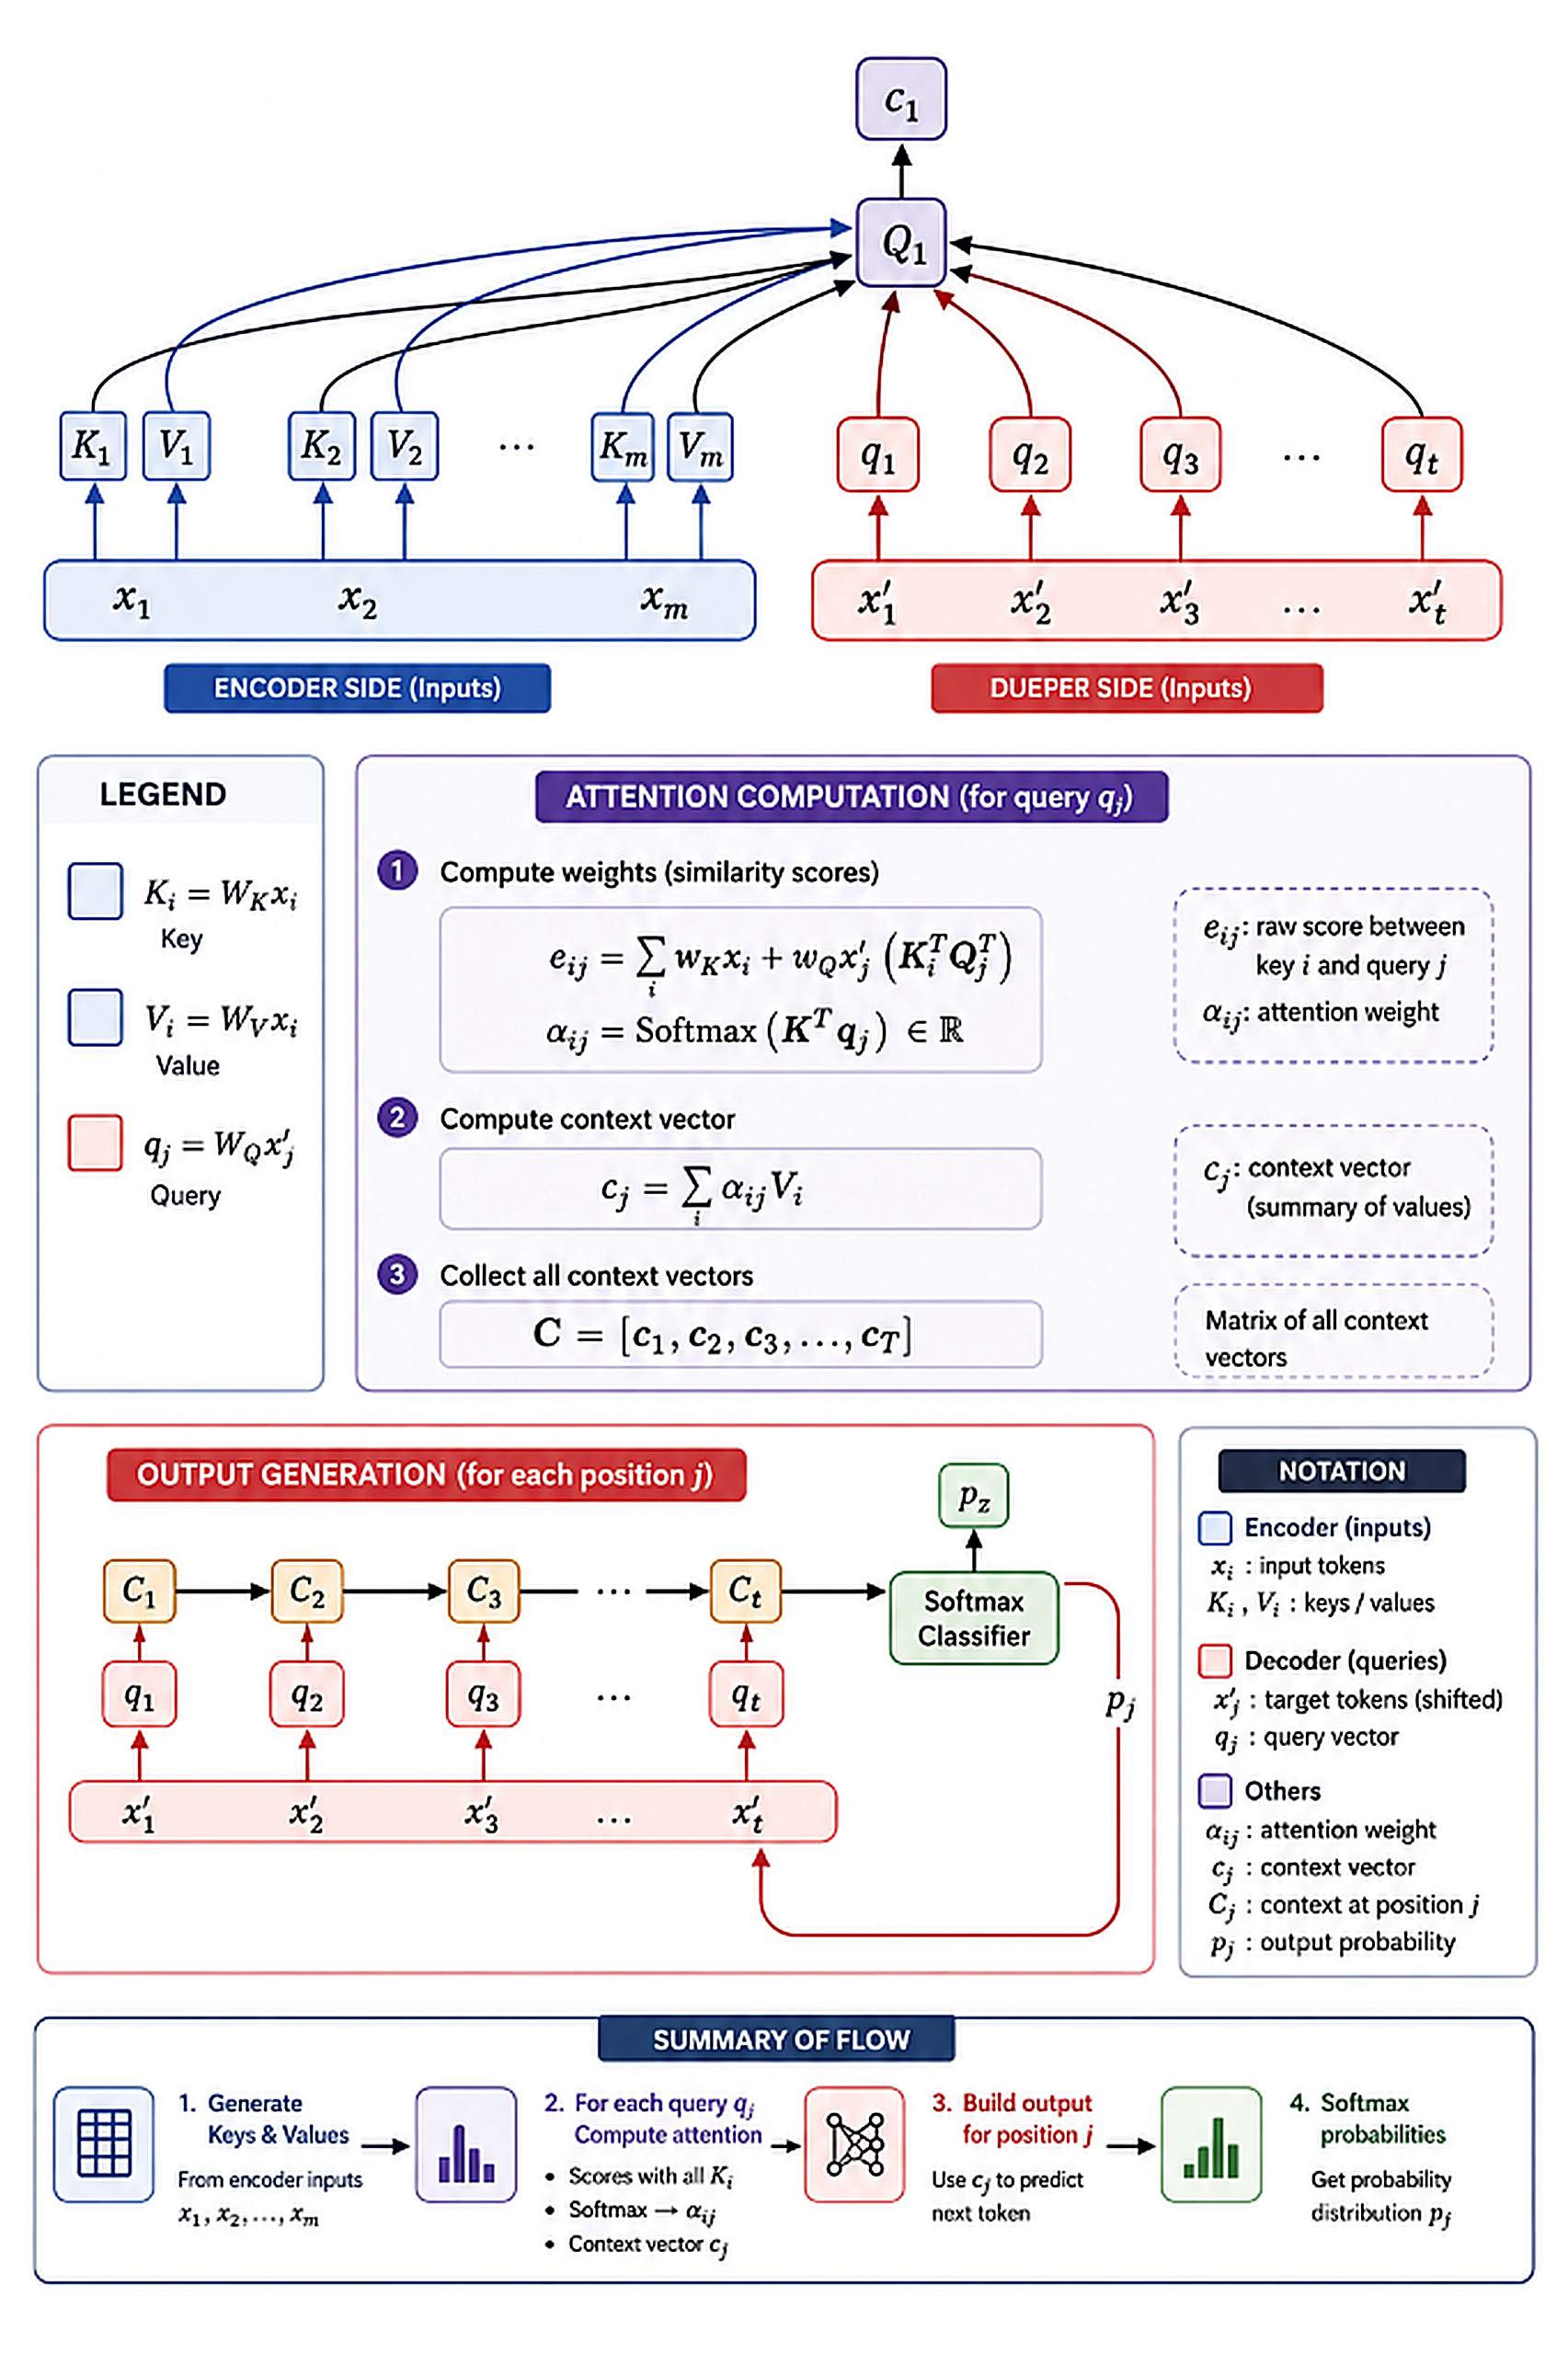
\includegraphics[width=0.85\textwidth]{figures/fig_5_attention_flow_pg121.png}
    \caption{Detailed computation flow of attention mechanisms operating over encoder and decoder inputs.}
    \label{fig:attention_flow_pg121}
\end{figure}

Key: $K_i = W_K x_i$ \\
Value: $V_i = W_V x_i$ \\
Query: $q_j = W_Q x_j'$

Compute weights:
\begin{equation}
\alpha_{ij} = \operatorname{softmax}_i\left(\frac{q_j K_i^T}{\sqrt{d_k}}\right)
\end{equation}

Compute Context Vector:
\begin{equation}
c_j = \sum_i \alpha_{ij} V_i, \quad C = [c_1, c_2, c_3, \dots, c_T]
\end{equation}

So Attention Layer: $C = \text{Attn}(x, x')$
\begin{itemize}
    \item Encoder inputs: $[x_1, x_2, x_3, \dots, x_m]$
    \item Decoder inputs: $[x_1', x_2', x_3', \dots, x_t']$
    \item Parameters: $W_Q, W_K, W_V$
\end{itemize}

Classical attention asks: \textit{Which encoder hidden states are important for this decoder state?} \\
Instead of directly comparing $h_i$ and $s_i$, we first project them into another space:
\begin{align}
q_t &= W_Q \cdot s_t \quad \text{(Query, obtained from decoder)} \\
K_i &= W_K \cdot h_i \quad \text{(Key, obtained from encoder)} \\
V_i &= W_V \cdot h_i \quad \text{(Value, obtained from encoder)}
\end{align}

\subsection{Why Do We Need \texorpdfstring{$Q, K, and V$}{Q, K, and V}?}
Why not compare with $h_i$ directly? Because different tasks need different notions of similarity. \\
For example, suppose “apple” sometimes means fruit, sometimes company.
\begin{itemize}
    \item The model learns $W_K$ to encode meaning.
    \item The model learns $W_Q$ to encode what we are looking for.
    \item The model learns $W_V$ to encode the information we finally want.
\end{itemize}

So Old Attention: Keys come from Encoder, Queries come from Decoder. \\
So let's come to the brilliant insight: \textit{Where do Queries really come from? Why not create them directly from the input?}

Instead of $q = W_Q s_i$, let's do:
\begin{align}
q &= W_Q x_i \quad \text{in the encoder} \\
K &= W_K x_i \\
V &= W_V x_i
\end{align}

Now: everything comes from the input itself:
\begin{itemize}
    \item No decoder state needed
    \item No encoder state needed
    \item Only embeddings
\end{itemize}

So that's what we call: \textbf{Self-Attention}.

In Self-Attention Layer: $C = \text{Attn}(X, X)$ \\
Input: $[x_1, x_2, \dots, x_m]$ \\
Parameters: $W_Q, W_K, W_V$

\begin{equation}
\alpha_i = \text{Softmax}(K^T q_i) \in \mathbb{R}^m
\end{equation}
\begin{equation}
c_i = V \cdot \alpha_i
\end{equation}
Output of Self-Attention layer: $[c_1, c_2, \dots, c_m]$.

This is the heart of the Transformer: Each word asks: \textit{Which other words help me understand myself?} \\
Example: “The animal didn't cross the street because it was tired”. \\
Token “it” creates Query and compares itself with every Key (e.g. animal: 0.8, street: 0.1 \dots). Output becomes mostly animal. This is exactly what Self-Attention computes.

\subsection{Mathematical Derivations}
Let $X = \begin{bmatrix} x_1 \\ x_2 \\ x_3 \\ \vdots \\ x_n \end{bmatrix}$. Project:
\begin{equation}
Q = X W_Q, \quad K = X W_K, \quad V = X W_V
\end{equation}
Similarity matrix: $S = Q K^T$ \\
Normalize: $A = \text{Softmax}(S)$ \\
Output: $C = A \cdot V$

The Full Equation:
\begin{equation}
\text{Attn}(Q, K, V) = \text{softmax}\left(\frac{Q K^T}{\sqrt{d_k}}\right) V
\end{equation}

Summary:
\begin{itemize}
    \item Classical attention lets a decoder query encoder representations.
    \item By generating Queries, Keys, and Values directly from the input embedding, we eliminate the need for recurrent hidden states.
    \item This leads to self-attention, where every token can attend to every other token in parallel.
    \item Self-attention becomes the fundamental building block of the Transformer.
    \item (Attention was originally developed for Seq2Seq RNN models, and self-attention for all RNN models, not necessarily Seq2Seq models).
\end{itemize}

\section{The "Attention Is All You Need" Paper Architecture}
The “Attention Is All You Need” paper, published by Vaswani et al. in 2017, introduced the Transformer, a novel neural network architecture that fundamentally changed sequence modeling. Unlike Seq2Seq models based on RNNs, LSTMs, and GRUs, the Transformer completely eliminates recurrence and relies solely on attention mechanisms to model dependencies between tokens. This design enables full parallel computation during training, significantly improves the modeling of long-range dependencies, and achieves superior computational efficiency.

The Transformer is built upon several key innovations, including Scaled Dot-Product Attention, Multi-Head Attention, Positional Encoding, Residual Connections, Layer Normalization, and Position-wise Feed-Forward Networks. These components are organized into an encoder-decoder architecture composed of stacked layers that learn increasingly rich contextual representations.

The Transformer has become the foundation of nearly all modern deep learning models for language, vision, speech, and multimodal learning: BERT, GPT, ViT, and LLMs.

\begin{figure}[htbp]
    \centering
    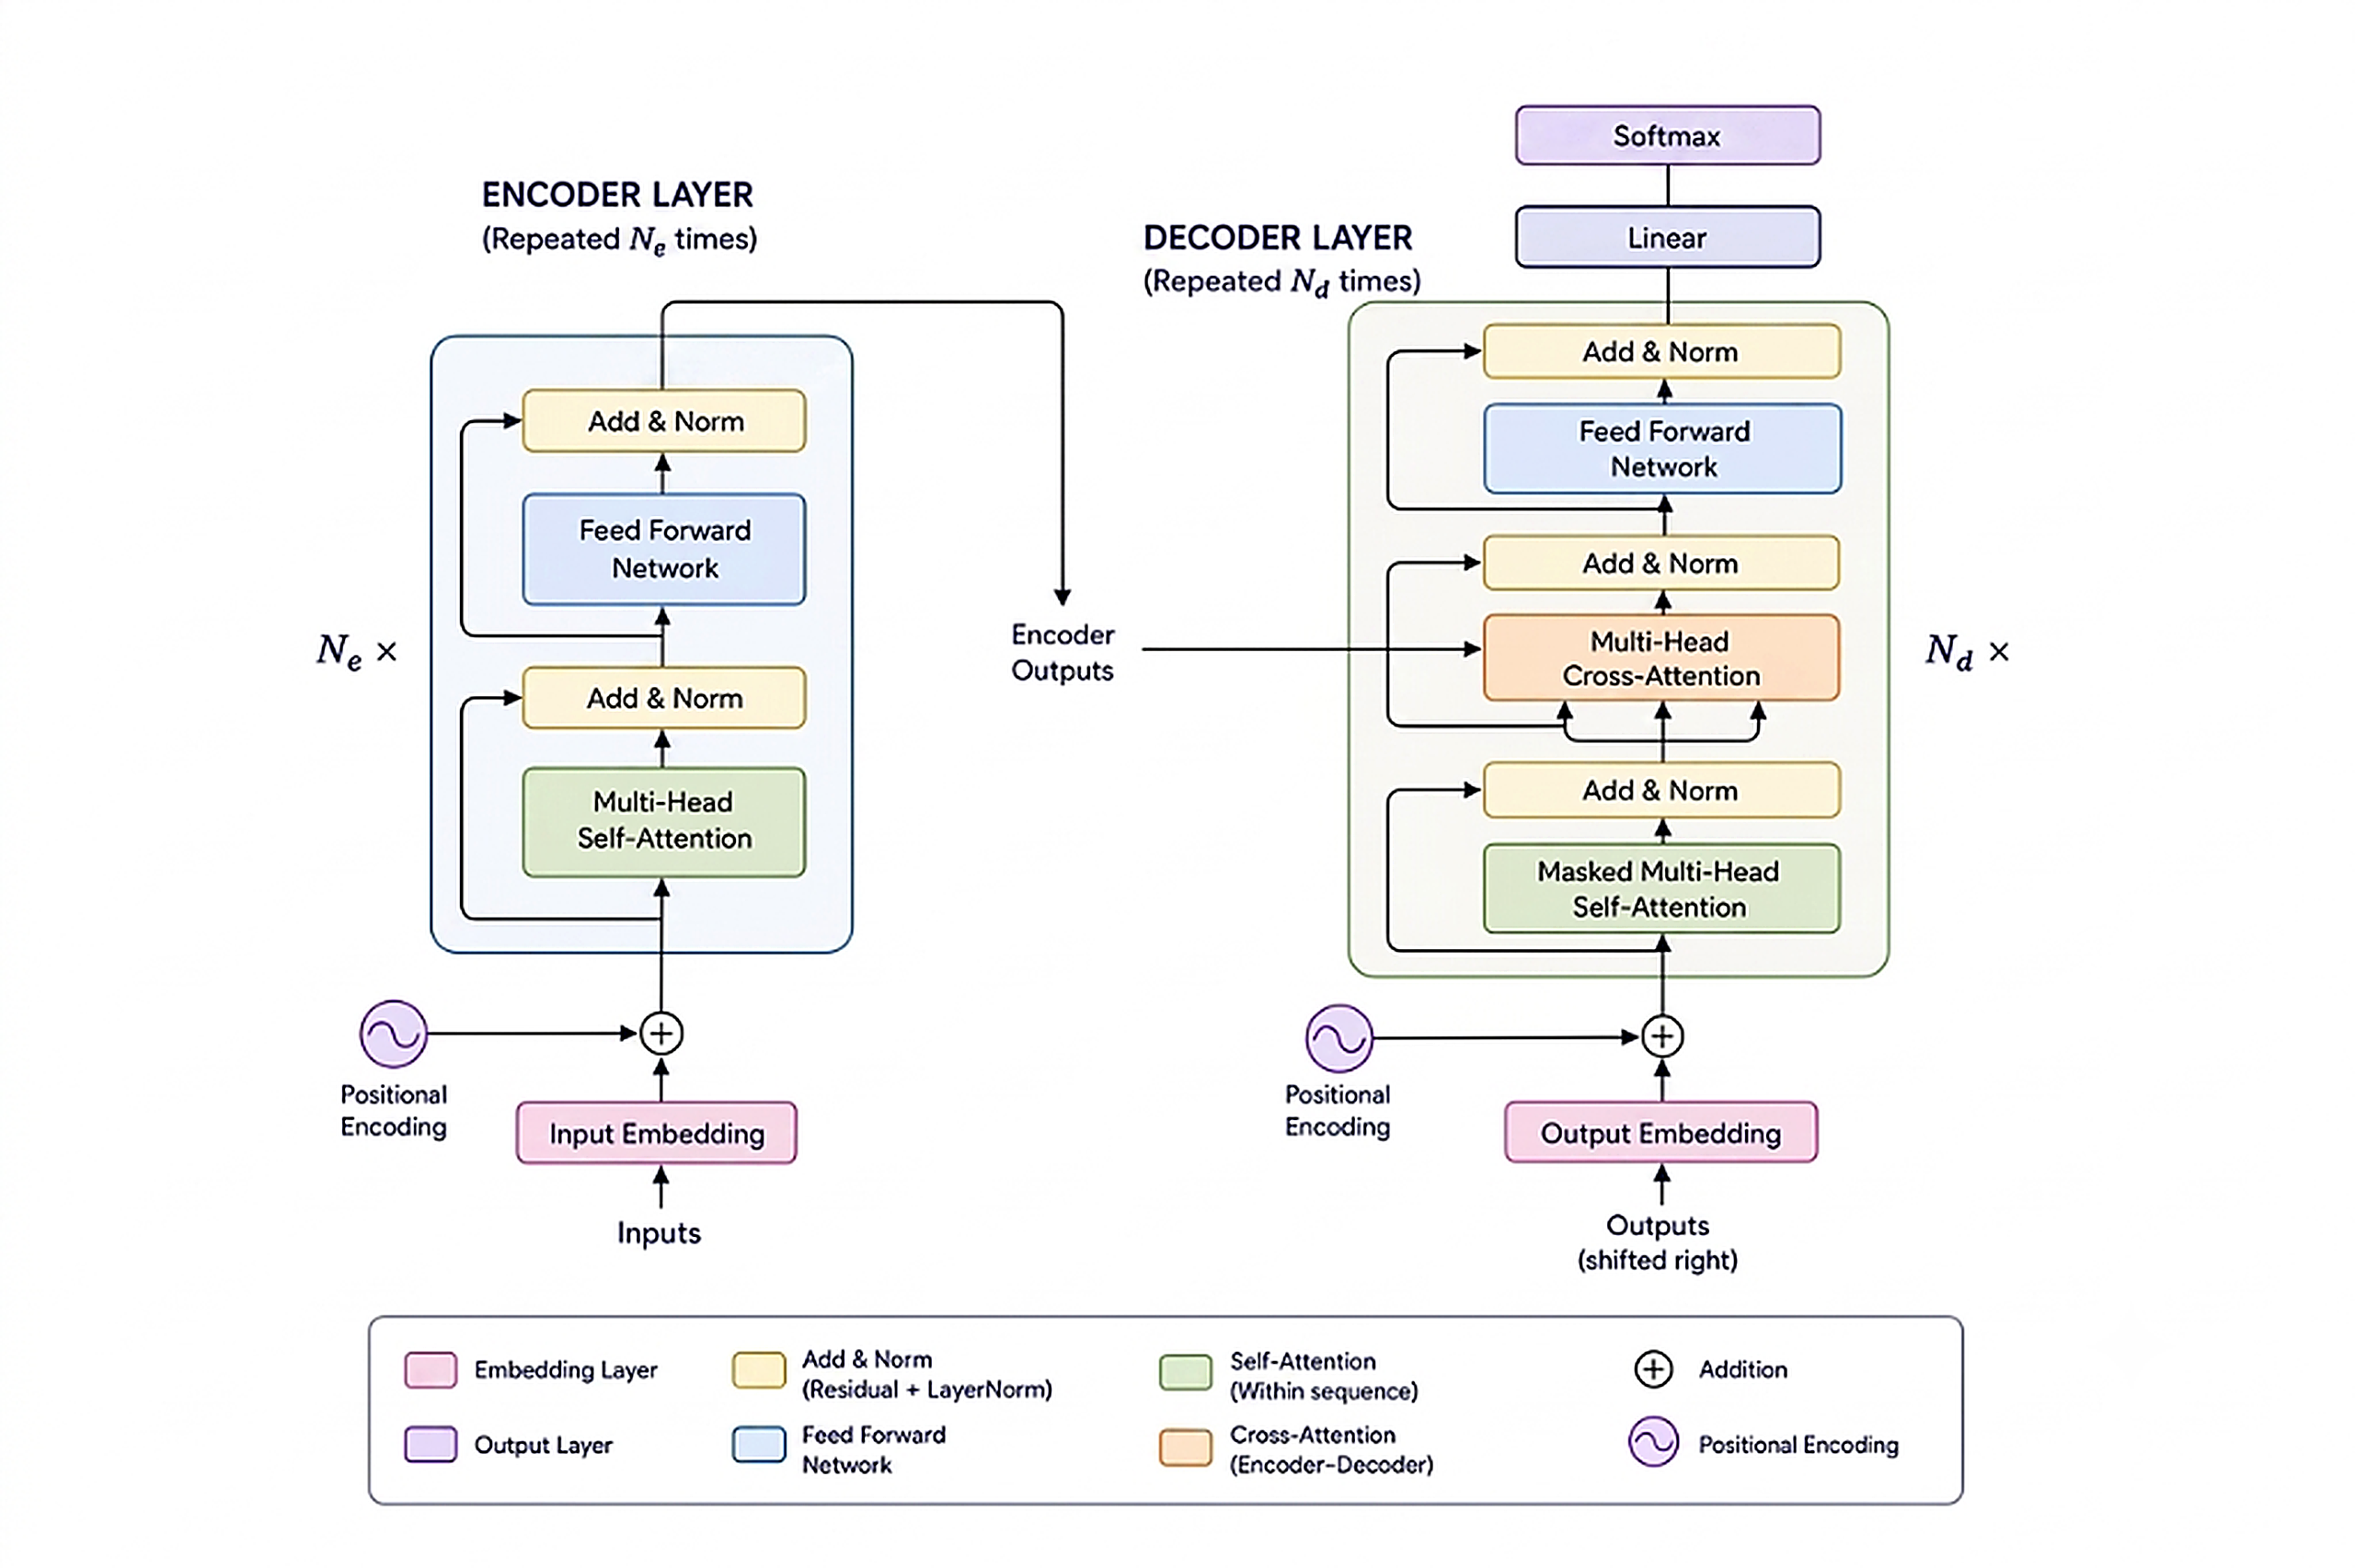
\includegraphics[width=0.88\textwidth]{figures/fig_5_transformer_architecture_pg128.png}
    \caption{The complete Transformer encoder-decoder model architecture.}
    \label{fig:transformer_architecture}
\end{figure}

\section{From Single-Head to Multi-Head Attention}
\subsection{Single-Head Self-Attention}
The Transformer begins with a single self-attention mechanism in which every token simultaneously acts as a query, key, and value. Given an input sequence $X \in \mathbb{R}^{n \times d_{model}}$, three learned linear projections generate the Query, Key, and Value matrices:
\begin{equation}
Q = X W_Q, \quad K = X W_K, \quad V = X W_V
\end{equation}
where $W_Q, W_K \in \mathbb{R}^{d_{model} \times d_k}$, and $W_V \in \mathbb{R}^{d_{model} \times d_v}$.

\begin{equation}
\text{Attention}(Q, K, V) = \text{Softmax}\left(\frac{Q K^T}{\sqrt{d_k}}\right) V
\end{equation}
where $Q K^T \in \mathbb{R}^{n \times n}$ contains the similarity between every pair of tokens.

\subsection{Why Divide by \texorpdfstring{$\sqrt{d_k}$}{sqrt(dk)}?}
The original Transformer divides the attention score by $\sqrt{d_k}$. Before applying Softmax, without this scaling factor, the variance of the dot products grows proportionally to $d_k$, causing Softmax to become highly saturated. Saturated probabilities produce extremely small gradients, slowing optimization and making training unstable. Dividing by $\sqrt{d_k}$ normalizes the variance of the attention scores, preserving stable gradients throughout training.

\begin{examplebox}[Numerical Comparison of Softmax Scaling]
Without scaling:
\begin{equation}
\text{Softmax}([16, 8, 0]) = [0.9997, 0.0003, 0.0000]
\end{equation}
The distribution is almost one-hot. The gradient of the Softmax $= 0.9997(1 - 0.9997) \approx 0.0003$. This is extremely small, hence learning is slow and gradients nearly vanish.

With scaling (e.g., dividing by $\sqrt{d_k} = \sqrt{64} = 8$):
\begin{equation}
\text{Softmax}([2, 1, 0]) = [0.665, 0.245, 0.090]
\end{equation}
Now the probabilities are much smoother: $0.665(1 - 0.665) = 0.223$. Training is therefore much more stable because useful gradients continue flowing through the network.
\end{examplebox}

\subsection{Multi-Head Attention}
A single attention head can learn only one similarity function at a time. To allow the model to capture multiple semantic relationships simultaneously, the Transformer employs Multi-Head Attention. Instead of learning one projection set, the model learns $h$ independent projection sets:
\begin{equation}
W_Q^i, W_K^i, W_V^i \quad \text{for } i = 1, \dots, h
\end{equation}

Each head computes $\text{head}_i = \text{Attention}(Q_i, K_i, V_i)$. \\
The outputs are concatenated: $H = \text{Concat}(\text{head}_1, \text{head}_2, \dots, \text{head}_h)$ and projected back into the model space:
\begin{equation}
\text{MultiHead}(Q, K, V) = \text{Concat}(\text{head}_1, \text{head}_2, \dots, \text{head}_h) W_O
\end{equation}
where $W_O \in \mathbb{R}^{h d_v \times d_{model}}$.

Example: $d_{model} = 512$ and $h = 8$, so $d_k = d_v = \frac{512}{8} = 64$.

\begin{figure}[htbp]
    \centering
    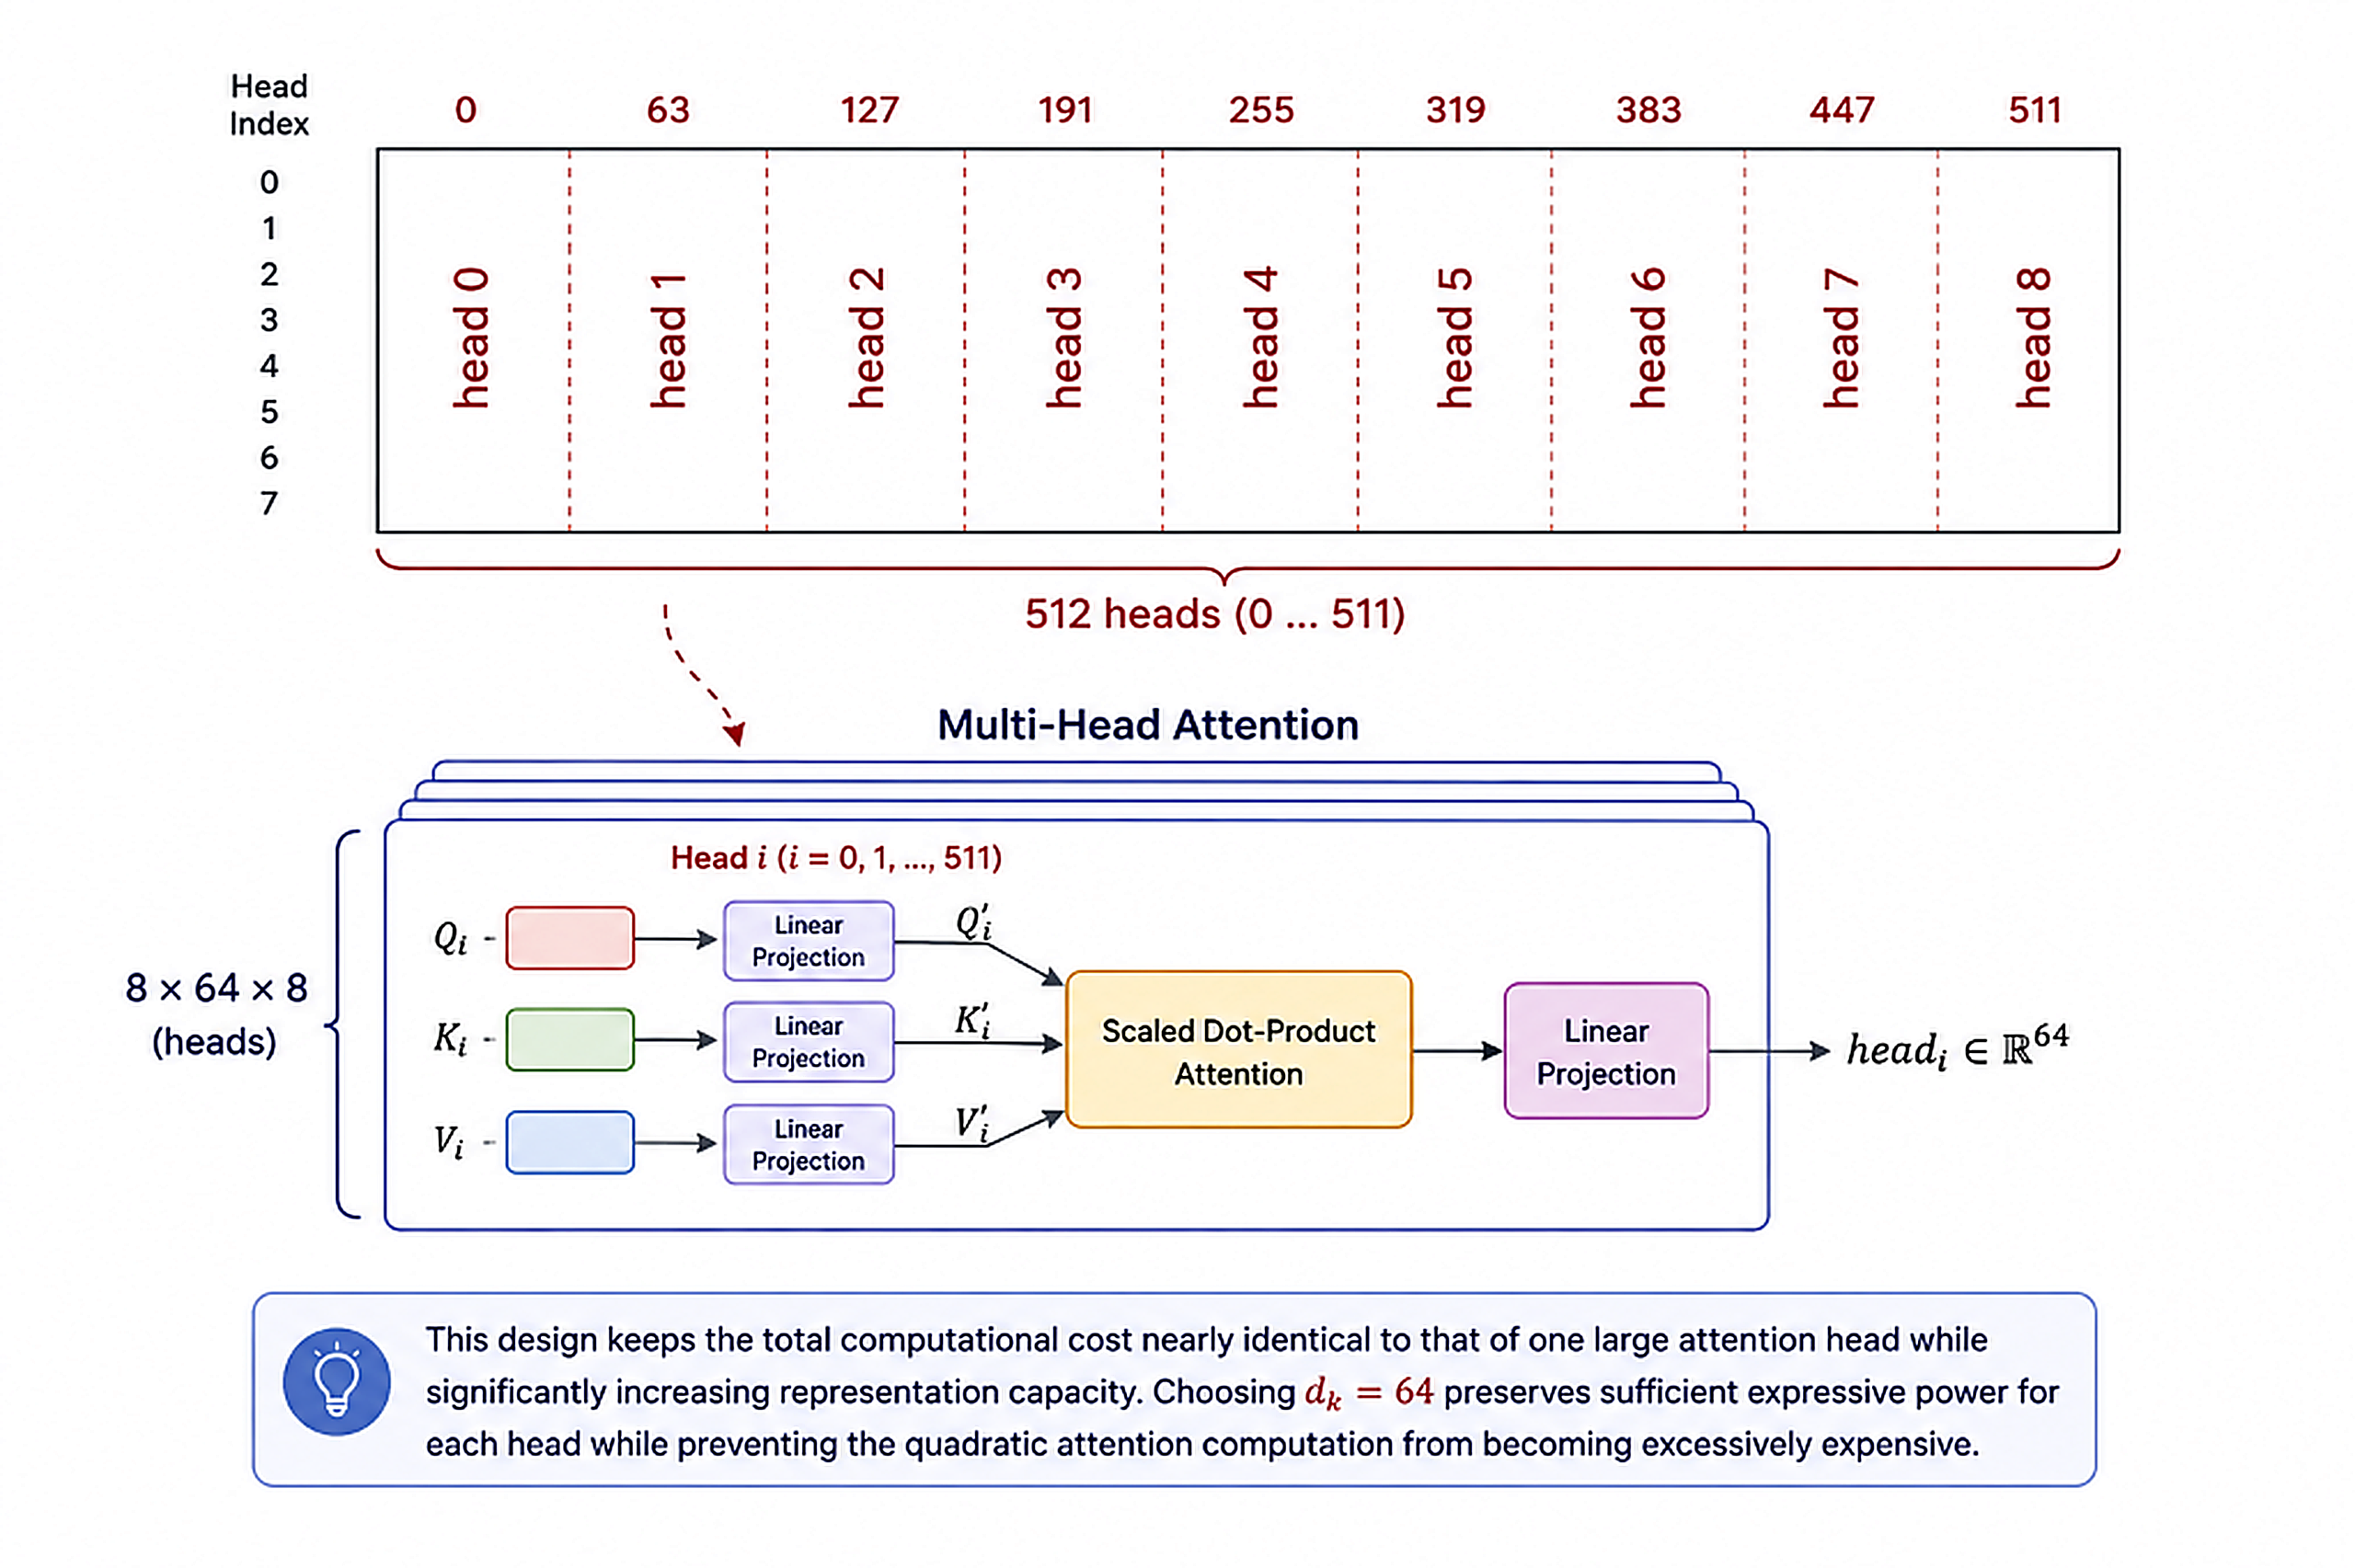
\includegraphics[width=0.92\textwidth]{figures/fig_5_multi_head_attention_pg132.png}
    \caption{Structural breakdown and linear projection flow in Multi-Head Attention.}
    \label{fig:multi_head_attention}
\end{figure}

\section{Positional Encoding}
Self-attention is permutation invariant because attention depends only on pairwise similarities and contains no information about token order. Consequently, positional information must be explicitly injected into the input representation.

The Transformer adds positional encodings directly to the token embeddings:
\begin{equation}
X' = X + PE
\end{equation}
where $X \in \mathbb{R}^{n \times d_{model}}$ and $PE \in \mathbb{R}^{n \times d_{model}}$.

Instead of learning position vectors, Transformer uses deterministic sinusoidal functions. For every position $pos$ and embedding dimension $i$:
\begin{align}
PE_{(pos, 2i)} &= \sin\left(\frac{pos}{10000^{2i/d_{model}}}\right) \\
PE_{(pos, 2i+1)} &= \cos\left(\frac{pos}{10000^{2i/d_{model}}}\right)
\end{align}
\begin{itemize}
    \item The even dimension: Use sinus function
    \item The odd dimension: Use cosinus function
\end{itemize}

Using sinusoidal functions provides unique positional representations while enabling the model to generalize to sequence lengths not observed during training, because nearby positions generate nearby vectors, and relative distances can also be inferred through linear operations.

\subsection{Why Different Frequencies?}
$10000^{2i/d_{model}}$ changes with the embedding dimension:
\begin{itemize}
    \item Low-dimension components have short wavelengths and vary rapidly with position.
    \item High-dimension components have long wavelengths and vary slowly.
\end{itemize}

\begin{figure}[htbp]
    \centering
    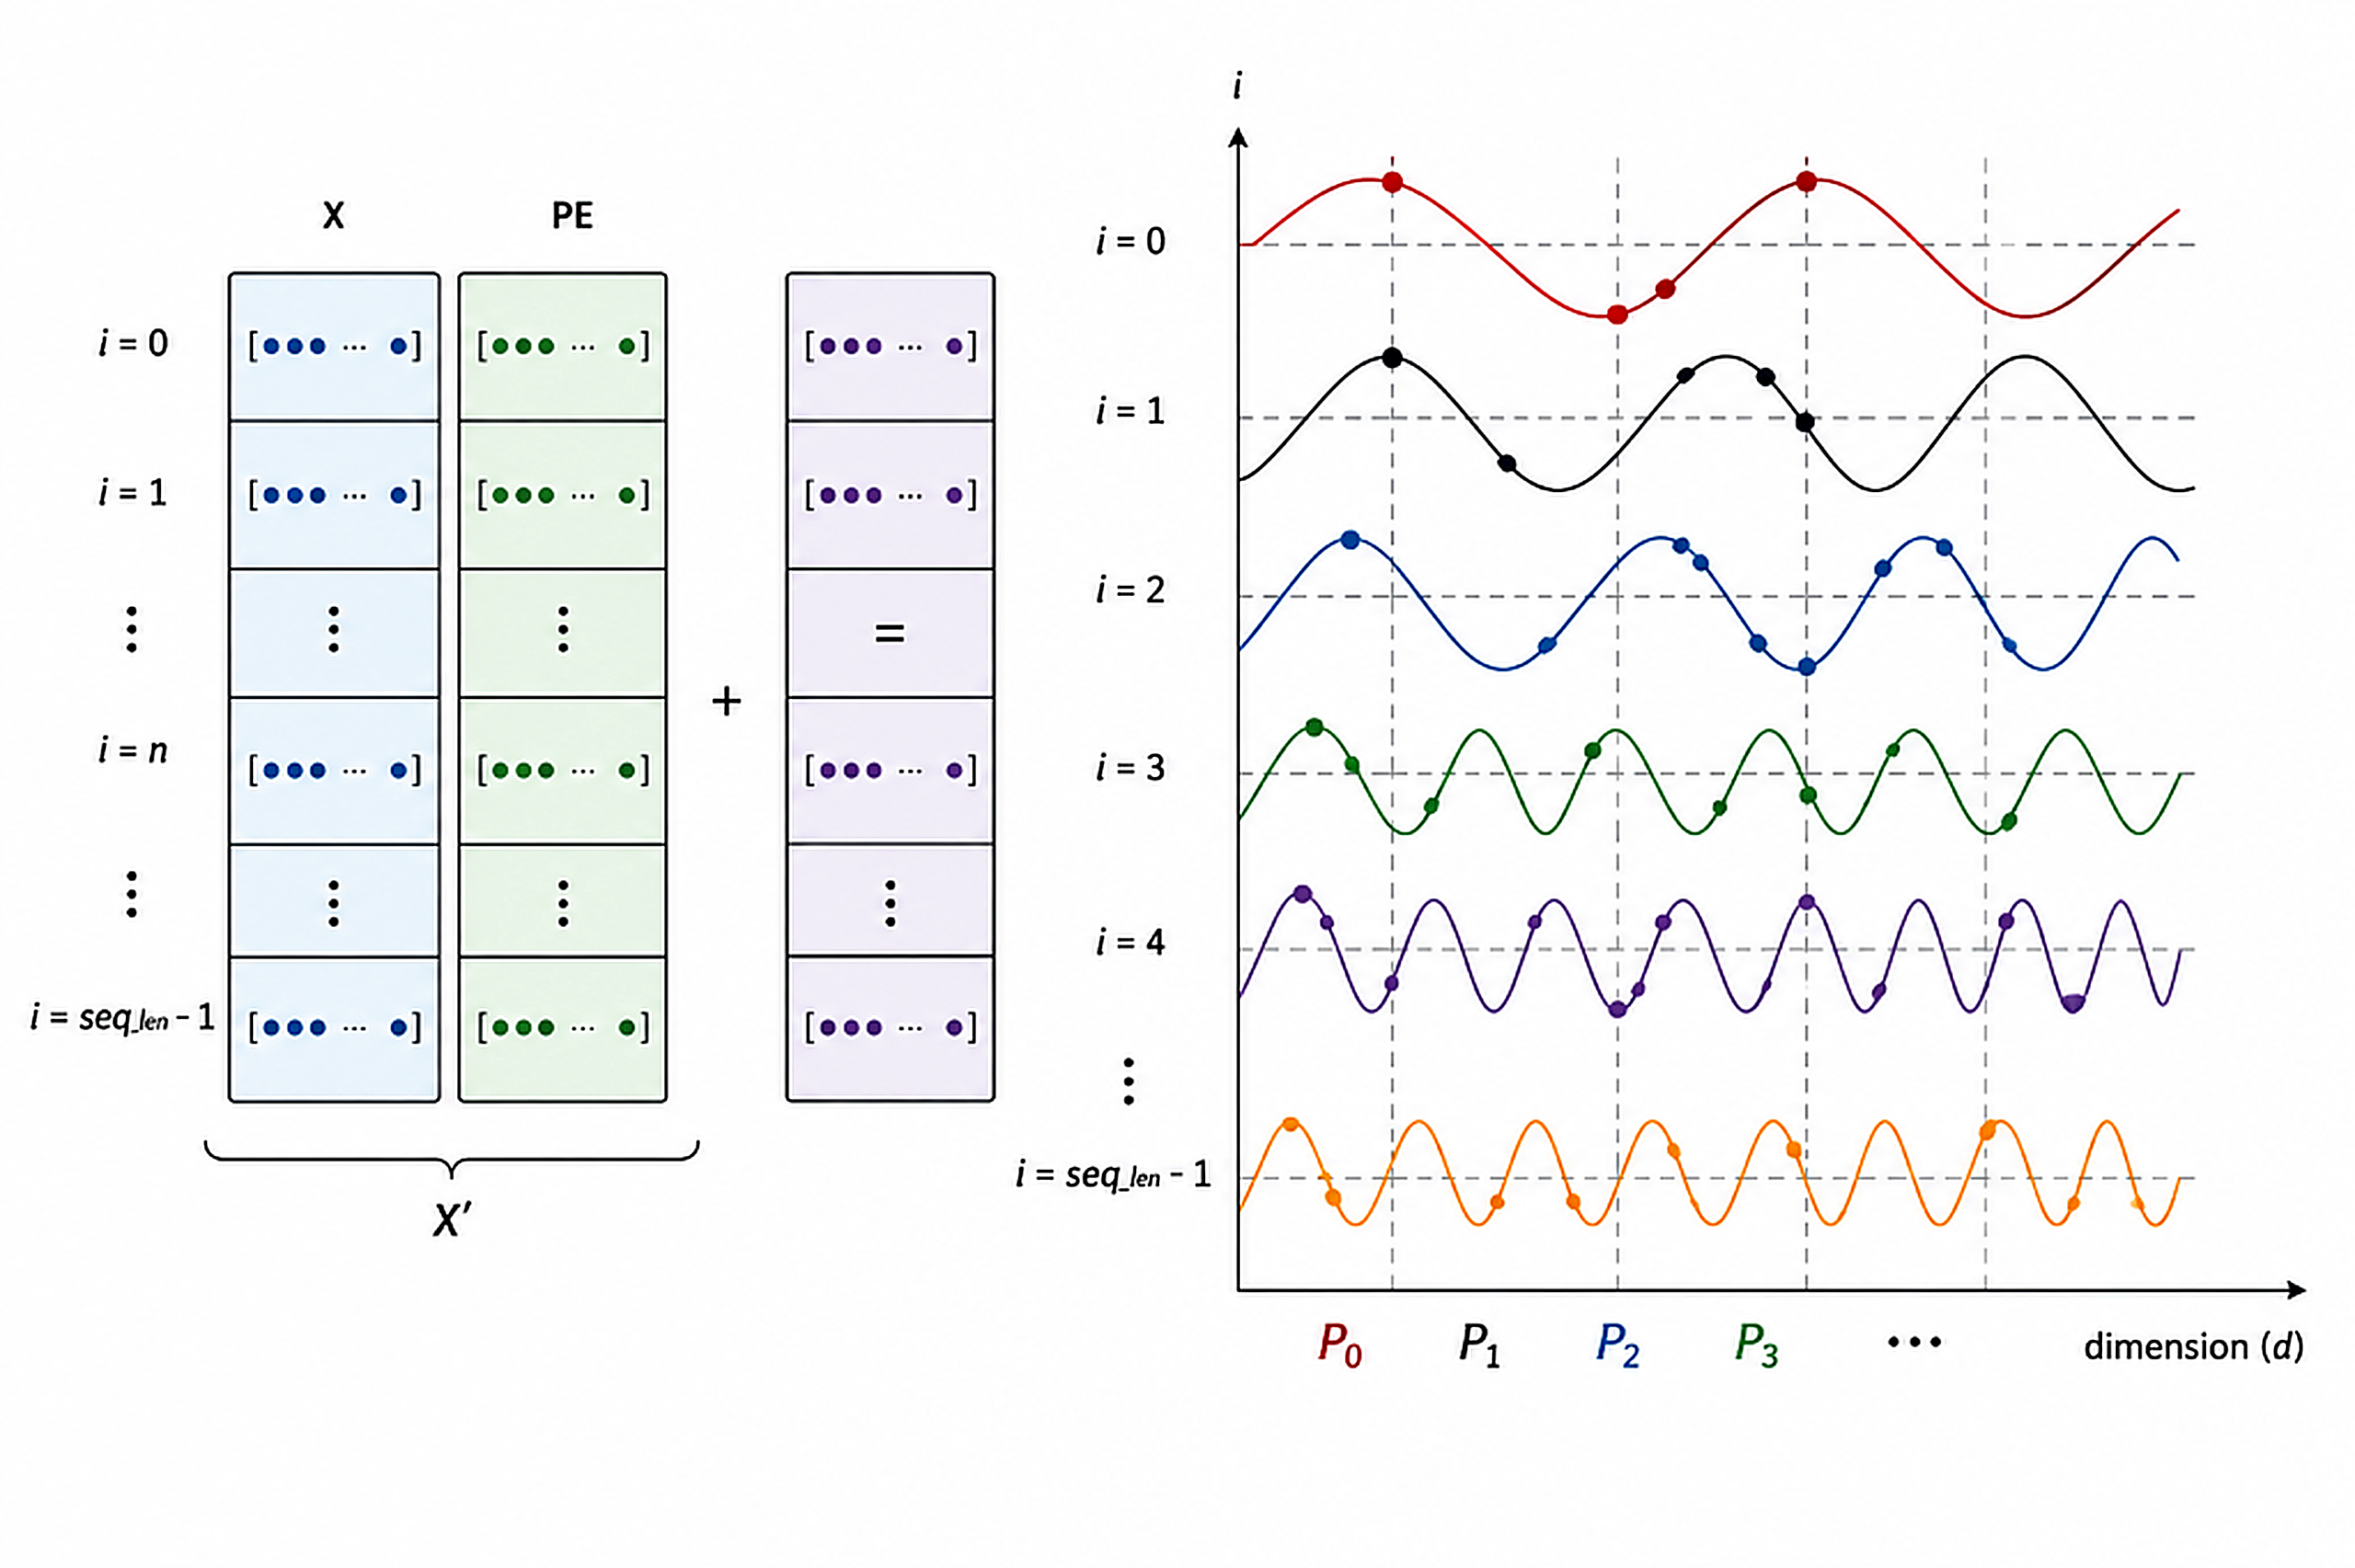
\includegraphics[width=0.88\textwidth]{figures/fig_5_positional_encoding_curves_pg134.png}
    \caption{Superposition of sinusoidal curves across embedding dimensions.}
    \label{fig:positional_curves}
\end{figure}

\begin{figure}[htbp]
    \centering
    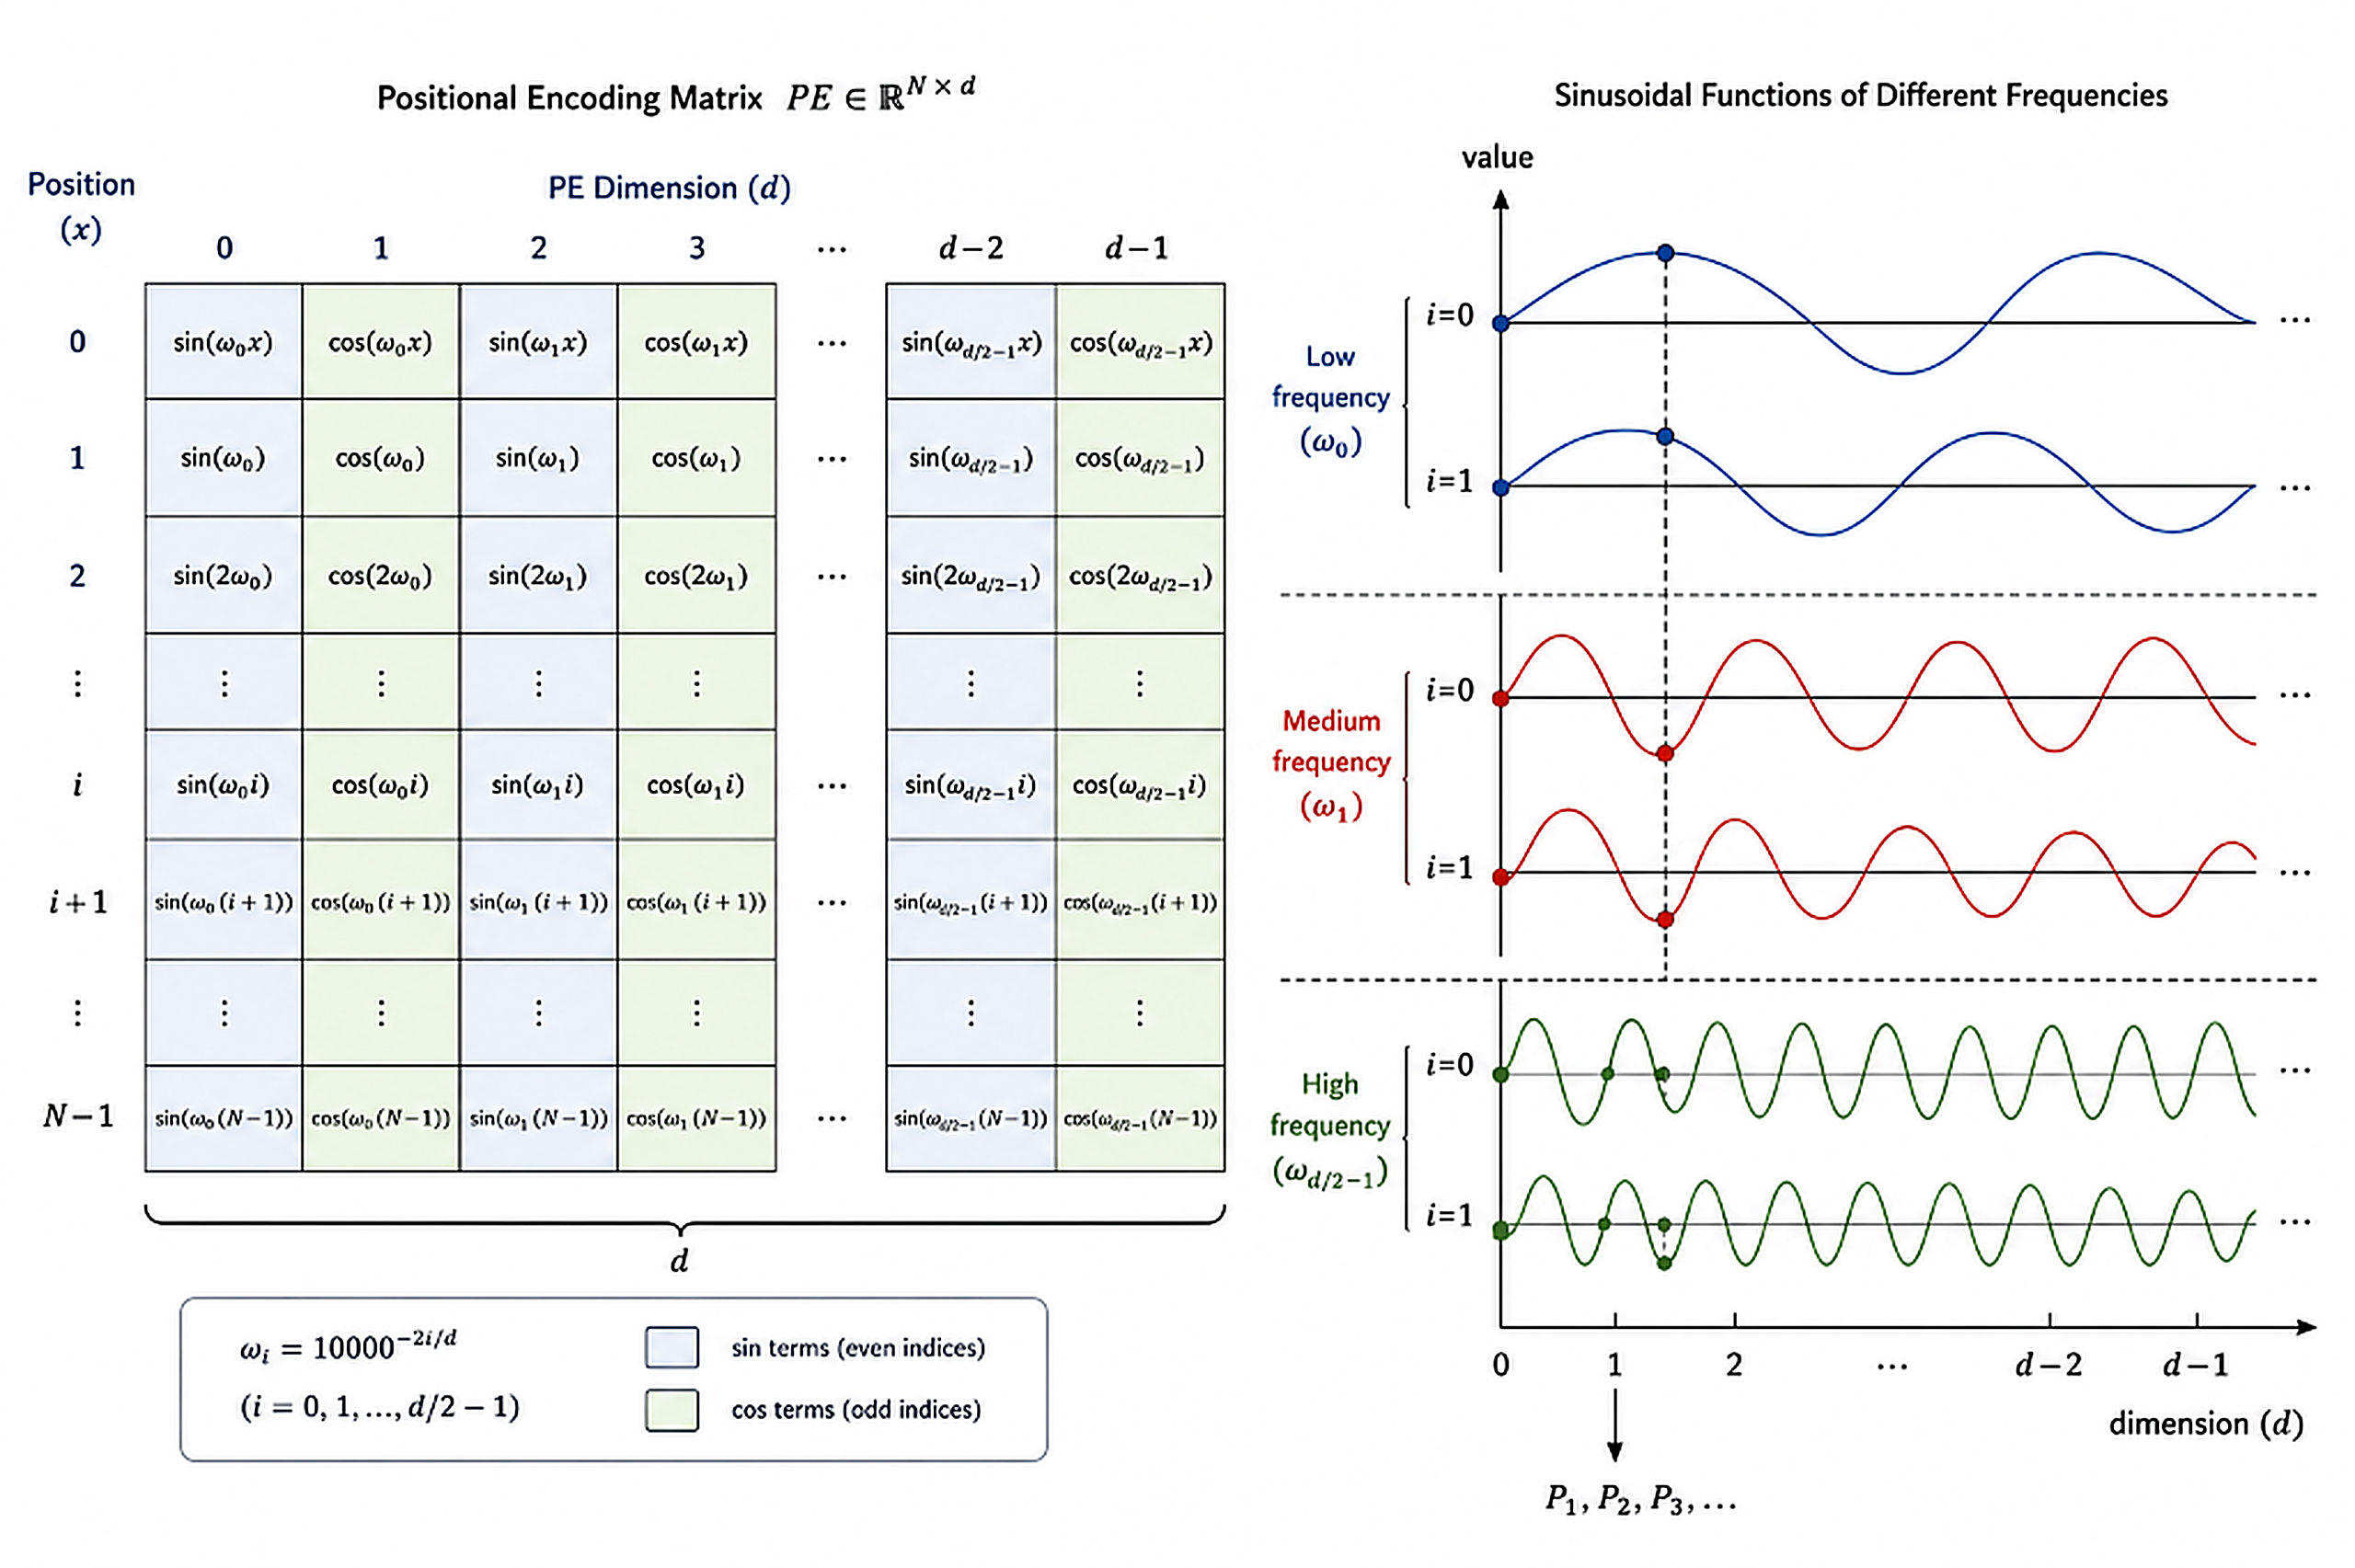
\includegraphics[width=0.88\textwidth]{figures/fig_5_positional_encoding_matrix_pg134.png}
    \caption{Structure of the Positional Encoding Matrix $PE \in \mathbb{R}^{N \times d}$.}
    \label{fig:positional_matrix}
\end{figure}

Example: $d_{model} = 8, pos = 3$. \\
The positional encoding vector becomes:
\begin{equation}
PE(3) = \left[ \sin(3), \cos(3), \sin(3/10), \cos(3/10), \sin(3/100), \cos(3/100), \sin(3/1000), \cos(3/1000) \right]
\end{equation}
Each pair of dimensions oscillates at a different frequency. Thus every position obtains a distinct vector.

\subsection{Why Sine and Cosine?}
\begin{enumerate}
    \item \textbf{Unique Representation}: Each position produces a different combination of sine and cosine values ($PE(pos_1) \neq PE(pos_2)$). For different positions, the model can distinguish every token location.
    \item \textbf{Smoothness}: Unlike one-hot position vectors, neighboring positions generate similar vectors. For example, $PE(20)$ is much closer to $PE(21)$ than $PE(200)$. This smooth transition makes optimization easier.
    \item \textbf{Relative Position Information} (The most important property): \\
    Using trigonometric identities:
    \begin{align}
    \sin(a+b) &= \sin(a)\cos(b) + \cos(a)\sin(b) \\
    \cos(a+b) &= \cos(a)\cos(b) - \sin(a)\sin(b)
    \end{align}
    Therefore, $PE(pos+k)$ can be expressed as a linear transformation of $PE(pos)$. This means the model can learn relationships such as next word and previous token.
    \item \textbf{Extrapolation to Longer Sequences}: Because the positional encoding is generated by a mathematical formula rather than learned parameters, it can be computed for positions beyond the training sequence length; however, successful extrapolation is not guaranteed.
\end{enumerate}

\subsection{Why Use Addition Instead of Concatenation?}
$X' = X + PE$. If concatenation were used instead, the dimensionality would increase (e.g. from 512 to 1024), doubling the size of the projection matrices and significantly increasing the number of parameters and computational cost.

Positional encoding enables the Transformer to model sequence order despite processing all tokens in parallel. By adding deterministic sinusoidal vectors to the input embeddings, the model receives explicit information about token positions while preserving the embedding dimensionality. The use of multiple sine and cosine frequencies produces unique, smooth, and mathematically structured representations that allow the model to infer both absolute position and relative distance. These encodings can be computed for positions beyond the training sequence length, although successful extrapolation is not guaranteed.

Although this method is elegant and parameter-free, it is rarely used in modern LLMs. Today, the most widely adopted technique is Rotary Position Embedding (RoPE), introduced in 2021. RoPE incorporates positional information by rotating the Query and Key vectors before computing attention, allowing the model to naturally capture relative positional relationships and perform better on long-context sequences.

\section{Rotary Position Embedding (RoPE)}
\begin{center}
\begin{tikzpicture}[
    node distance=1.2cm, 
    auto, 
    >=stealth, 
    font=\sffamily\bfseries\small,
    mainnode/.style={draw=primaryblue, fill=boxbg, text=primaryblue, rounded corners=4pt, inner sep=6pt, line width=0.8pt},
    secnode/.style={draw=secondaryblue, fill=secondaryblue!12, text=primaryblue, rounded corners=4pt, inner sep=6pt, line width=0.8pt},
    rotnode/.style={draw=accentred, fill=accentred!12, text=accentred!90!black, rounded corners=4pt, inner sep=6pt, line width=0.8pt},
    outnode/.style={draw=primaryblue, fill=boxbg, text=primaryblue, rounded corners=4pt, inner sep=6pt, line width=0.8pt}
]
    \node [mainnode] (emb) {Embedding};
    \node [secnode, right=of emb] (proj) {Linear Projection};
    \node [mainnode, above right=0.3cm and 0.8cm of proj] (Q) {$\mathbf{Q}$};
    \node [mainnode, below right=0.3cm and 0.8cm of proj] (K) {$\mathbf{K}$};
    \node [rotnode, right=of Q] (rotQ) {Rotate $\mathbf{Q}'$};
    \node [rotnode, right=of K] (rotK) {Rotate $\mathbf{K}'$};
    \node [outnode, right=1.6cm of rotQ, yshift=-0.8cm] (attn) {$\text{Softmax}\left(\frac{\mathbf{Q}' \mathbf{K}'^T}{\sqrt{d_k}}\right)$};
    
    \draw [->, line width=1.1pt, primaryblue] (emb) -- (proj);
    \draw [->, line width=1.1pt, primaryblue] (proj) |- (Q);
    \draw [->, line width=1.1pt, primaryblue] (proj) |- (K);
    \draw [->, line width=1.1pt, primaryblue] (Q) -- (rotQ);
    \draw [->, line width=1.1pt, primaryblue] (K) -- (rotK);
    \draw [->, line width=1.1pt, primaryblue] (rotQ) -| (attn);
    \draw [->, line width=1.1pt, primaryblue] (rotK) -| (attn);
\end{tikzpicture}
\end{center}

Example: position $p = 3$, angle $\theta = 30^\circ$, Query vector $Q = \begin{bmatrix} 2 \\ 1 \end{bmatrix}$. \\
The rotation matrix is:
\begin{equation}
R = \begin{bmatrix} \cos 30^\circ & -\sin 30^\circ \\ \sin 30^\circ & \cos 30^\circ \end{bmatrix} = \begin{bmatrix} 0.866 & -0.5 \\ 0.5 & 0.866 \end{bmatrix}
\end{equation}

Multiply:
\begin{equation}
Q' = R Q = \begin{bmatrix} 0.866 & -0.5 \\ 0.5 & 0.866 \end{bmatrix} \begin{bmatrix} 2 \\ 1 \end{bmatrix} = \begin{bmatrix} 1.232 \\ 1.866 \end{bmatrix}
\end{equation}
The rotation preserves the vector's norm while incorporating position-dependent information.

\begin{advbox}[Advantages of RoPE]
\begin{itemize}
    \item Captures relative positions naturally
    \item Better performance on long-context tasks
    \item No additional trainable parameters
    \item Computationally efficient
    \item Used in most modern LLMs (e.g., LLaMA, Qwen, Gemma, DeepSeek)
\end{itemize}
\end{advbox}

\section{Position-wise Feed Forward Network}
Forward Network Transforms each token independently:
\begin{equation}
\text{FFN}(x) = W_2 \sigma(W_1 x + b_1) + b_2
\end{equation}
Dimension flow: $512 \to 2048 \to 512$. \\
$W_1 \in \mathbb{R}^{512 \times 2048}, \quad W_2 \in \mathbb{R}^{2048 \times 512}$.

\section{Residual Connections And Add \& Norm}
Deep neural networks become increasingly difficult to optimize because gradients vanish as depth increases. To alleviate this problem, every sub-layer employs a residual connection:
\begin{equation}
y = x + F(x)
\end{equation}
allowing gradients to flow directly through identity mappings.

Immediately after the residual addition, Layer Normalization is applied:
\begin{equation}
\text{LayerNorm}(x + F(x))
\end{equation}
forming the well-known Add \& Norm Operation.

Residual Connections improve optimization, while normalization stabilizes the distribution of intermediate activations, accelerates convergence, and reduces sensitivity to parameter initialization.

\subsection{Layer Normalization}
Unlike Batch Normalization, which computes statistics across the batch dimension, Layer Normalization normalizes each token independently across its feature dimensions:
\begin{equation}
\text{LayerNorm}(x) = \gamma \frac{x - \mu}{\sqrt{\sigma^2 + \epsilon}} + \beta
\end{equation}
This independence from batch statistics makes Layer Normalization particularly suitable for variable-length sequences and autoregressive inference.

\section{Transformer Encoder}
The primary objective of the encoder is not generate output tokens. Instead, its role is to transform the input sequence into a set of context-aware representation that capture the semantic and syntactic relationships among all tokens. These contextual representations serve as the knowledge base from which the decoder later generates the target sequence.

Unlike an RNN encoder, which compresses information sequentially into hidden states, the Transformer encoder processes the entire sequence simultaneously through stacked attention layers, allowing every token to directly exchange information with every other token.

The output vector now contains contextual information from the entire sentence rather than representing only the corresponding token.

The output has exactly the same dimensions as the input:
\begin{equation}
X \in \mathbb{R}^{n \times 512} \longrightarrow U \in \mathbb{R}^{n \times 512}
\end{equation}
$n$: sequence length (tokens).

\subsection{Encoder Workflow and Architecture}
\textbf{1. Input to encoder:}
\begin{enumerate}
    \item Tokenization
    \item Embedding
    \item Positional Encoding
\end{enumerate}

Therefore the encoder receives:
\begin{equation}
X = \begin{bmatrix} x_1 \\ x_2 \\ \vdots \\ x_n \end{bmatrix} \in \mathbb{R}^{n \times 512}
\end{equation}

\textbf{2. Encoder Architecture:} \\
The original Transformer stacks $N = 6$ identical encoder blocks. Each block has exactly the same architecture but different learned parameters:
\begin{align}
U^{(0)} &= X \\
U^{(\ell)} &= \text{Encoder Block}^{(\ell)}\left(U^{(\ell-1)}\right), \quad \ell = 1, \dots, 6 \\
\text{The final encoder output is } U &= U^{(6)}
\end{align}

\subsection{Encoder Block Operations}
Each encoder block performs four operations sequentially: \\
$\text{Multi-Head Self-Attention} \longrightarrow \text{Add \& Norm} \longrightarrow \text{Feed Forward Network} \longrightarrow \text{Add \& Norm}$.

Although the dimensionality never changes, the representation becomes increasingly richer after every block.

\textbf{Step 1: Multi-Head Self-Attention} \\
The block first compute:
\begin{equation}
Q = X W_Q, \quad K = X W_K, \quad V = X W_V
\end{equation}
Attention produces:
\begin{equation}
H = \text{MultiHead}(Q, K, V)
\end{equation}
Dimension: $X \in \mathbb{R}^{n \times 512} \implies H \in \mathbb{R}^{n \times 512}$. \\
Every token now contains information collected from all other tokens.

\textbf{Step 2: Add \& Norm} \\
The attention output is added back to its input:
\begin{equation}
R_1 = X + H
\end{equation}
Layer Normalization is then applied:
\begin{equation}
Z = \text{LayerNorm}(R_1) \in \mathbb{R}^{n \times 512}
\end{equation}
The residual path preserves information from previous layers while normalization stabilizes optimization.

\textbf{Step 3: Feed Forward Network} \\
Each token independently passes through the same feed-forward network:
\begin{align}
F &= \text{FFN}(Z) \\
\text{FFN}(x) &= W_2 \text{ReLU}(W_1 x + b_1) + b_2
\end{align}
First layer: $512 \to 2048$, Second layer: $2048 \to 512$. \\
$Z \in \mathbb{R}^{n \times 512}$.

\textbf{Step 4: Add \& Norm} \\
A residual connection is applied:
\begin{equation}
R_2 = Z + F, \quad U = \text{LayerNorm}(R_2) \in \mathbb{R}^{n \times 512}
\end{equation}
This completes one encoder block.

\textbf{3. Stacking Encoder Blocks:} \\
The output of one encoder block immediately becomes the input of the next:
\begin{equation}
U^{(1)} \to U^{(2)} \to \dots \to U^{(6)}
\end{equation}
No block change tensor size $\in \mathbb{R}^{n \times 512}$.

Each successive block refines the contextual representation by repeatedly combining global information through attention and non-linear feature transformations through the feed-forward network.

\subsection{Encoder Output}
After the sixth encoder block, the encoder produces:
\begin{equation}
U = \begin{bmatrix} u_1 \\ u_2 \\ \vdots \\ u_n \end{bmatrix} \in \mathbb{R}^{n \times 512}
\end{equation}
Each vector $u_i$ now is a contextual representation that encodes information about the entire input sequence. Every token representation has been updated through multiple rounds of self-attention, allowing it to capture long-range dependencies and global context.

\section{Transformer Decoder}
The decoder is responsible for generating the target sequence one token at a time. The encoder built contextual representations of the input. The decoder uses these representation to predict the next output token autoregressively. At each decoding step, it conditions its prediction on two sources of information.

Consequently, the decoder learns the conditional probability distribution:
\begin{equation}
P(y_1, \dots, y_T \mid x_1, \dots, x_n) = \prod_{t=1}^T P(y_t \mid y_{<t}, X)
\end{equation}
$X$: the source sequence \\
$y_{<t}$: all previously generated target tokens.

Unlike the encoder, the decoder cannot process all target tokens independently during inference because each prediction depends on the previous ones.

\subsection{Decoder Architecture}
The original Transformer stacks $N = 6$ identical decoder block. Each block consists of: \\
$\text{Masked Multi-Head Self-Attention} \longrightarrow \text{Add \& Norm} \longrightarrow \text{Encoder-Decoder Attention} \longrightarrow \text{Add \& Norm} \longrightarrow \text{Feed Forward Network} \longrightarrow \text{Add \& Norm}$.

\subsection{Decoder Block Breakdown}
\textbf{Step 1: Masked Multi-Head Self-Attention} \\
Attention is computed as:
\begin{equation}
\text{Attention} = \text{Softmax}\left(\frac{Q K^T + M}{\sqrt{d_k}}\right) V
\end{equation}

Mask $M$:
\begin{equation}
\begin{bmatrix}
0.31 & 0.36 & 0.55 & 0.02 & 0.3 \\
0.25 & 0.13 & 0.21 & 0.01 & 0.17 \\
0.26 & 0.23 & 0.35 & 0.01 & 0.22 \\
0.01 & 0.04 & 0.07 & 0.0 & 0.02 \\
0.14 & 0.13 & 0.20 & 0.01 & 0.12
\end{bmatrix}
+
\begin{bmatrix}
0 & -\infty & -\infty & -\infty & -\infty \\
0 & 0 & -\infty & -\infty & -\infty \\
0 & 0 & 0 & -\infty & -\infty \\
0 & 0 & 0 & 0 & -\infty \\
0 & 0 & 0 & 0 & 0
\end{bmatrix}
=
\begin{bmatrix}
0.31 & -\infty & -\infty & -\infty & -\infty \\
0.25 & 0.13 & -\infty & -\infty & -\infty \\
0.26 & 0.23 & 0.35 & -\infty & -\infty \\
0.01 & 0.04 & 0.07 & 0.0 & -\infty \\
0.14 & 0.13 & 0.20 & 0.01 & 0.12
\end{bmatrix}
\end{equation}
Thus, the token at position $i$ can only attend to itself and all previous, but never to future tokens.

This masking mechanism prevents information leakage during training, ensuring that the decoder learns to predict the next token using only the previously generated content.

* The reason for using $-\infty$: we want the masked positions to receive exactly zero attention probability after applying Softmax, e.g., $\text{Softmax}([2, 1, -\infty]) = [0.665, 0.335, 0]$.

\textbf{Step 2: Add \& Norm} \\
Residual connection: $R_1 = Y + H, \quad Z = \text{LayerNorm}(R_1) \in \mathbb{R}^{t \times 512}$.

\textbf{Step 3: Encoder-Decoder Attention (Cross-Attention)} \\
This is the only operation that connects the decoder to the encoder. Unlike self-attention, the queries originate from the decoder, and the keys and values originate from the encoder output:
\begin{align}
Q &= Z W_Q \\
K &= U W_K \\
V &= U W_V
\end{align}
The attention becomes: $\text{Attention}(Q, K, V) = \text{Softmax}\left(\frac{Q K^T}{\sqrt{d_k}}\right) V$. \\
Output $C \in \mathbb{R}^{t \times 512}$ where $Q \in \mathbb{R}^{t \times 64}, K \in \mathbb{R}^{n \times 64}, V \in \mathbb{R}^{n \times 64}$ ($512/8 = 64$).

Unlike self-attention, where each token attends to the target sequence itself, cross-attention enables every decoder position to retrieve the most relevant information from the encoded source sequence.

\textbf{Step 4: Add \& Norm} \\
The output of the cross-attention is combined with the residual connection:
$R_2 = Z + C, \quad D_1 = \text{LayerNorm}(R_2) \in \mathbb{R}^{t \times 512}$.

\textbf{Step 5: Feed Forward Network} \\
Each decoder representation is independently transformed through the position-wise feed-forward network:
\begin{equation}
\text{FFN}(x) = W_2 \text{ReLU}(W_1 x + b_1) + b_2
\end{equation}
$512 \to 2048 \to 512$. Applied to the entire sequence: $t \times 512 \to t \times 2048 \to t \times 512$.

\textbf{Step 6: Add \& Norm} \\
The final residual connection is computed: $R_3 = \text{FFN} + R_2$, $D = \text{LayerNorm}(R_3)$. \\
This is complete one decoder block.

\subsection{Stacking Decoder Blocks and Prediction}
\textbf{Stacking Decoder Blocks:} \\
The Transformer stacks 6 decoder blocks:
\begin{align}
D^{(0)} &= Y \\
D^{(\ell)} &= \text{Decoder Block}^{(\ell)}\left(D^{(\ell-1)}, U\right), \quad \ell = 1, \dots, 6
\end{align}
The encoder output is shared by every decoder block, while the decoder representation is progressively refined.

\textbf{Final Decoder Output:} \\
After the sixth decoder block, $D \in \mathbb{R}^{t \times 512}$. \\
This matrix contains contextual representations of every generated target token, enriched by both the previously generated target sequence and the encoded source sequence. However, these vectors are not yet predicted words.

To produce the final prediction, each decoder output vector is passed through a linear projection:
\begin{equation}
Z = D W_{voc} + b, \quad W_{voc} \in \mathbb{R}^{512 \times |V|}
\end{equation}
$|V|$ is the vocabulary size: vocabulary is the set of all tokens that the model knows and can predict.

The resulting logits $Z \in \mathbb{R}^{t \times |V|}$ are converted into probabilities using $P = \text{Softmax}(Z)$. The token with the highest probability becomes the next generated token.

\section{Key-Value Cache (KV Cache)}

The Primary Goal of a Transformer during inference is to generate One Token at a time. This Process is Known as autoregressive Generation, Meaning that each newly generated Token depends on all Previously generated tokens.

Unlike training, where the entire target Sequence is available simultaneously, inference has access only to The Tokens that have already been Generated, Therefore, The model must repeatedly execute the decoder every new token until the Sequence is complete.

Suppose we want The model to Generate the Sentence: \\


\textit{The cat is sleeping on the sofa.}

\begin{center}
\begin{tabular}{l l}
$\langle \text{BOS} \rangle$
& $\rightarrow$ Predict ``The'' \\[4pt]

$\langle \text{BOS} \rangle$ The
& $\rightarrow$ Predict ``cat'' \\[4pt]

$\langle \text{BOS} \rangle$ The cat
& $\rightarrow$ Predict ``is'' \\[4pt]

$\langle \text{BOS} \rangle$ The cat is
& $\rightarrow$ Predict ``sleeping'' \\[4pt]

$\langle \text{BOS} \rangle$ The cat is sleeping
& $\rightarrow$ Predict ``on'' \\[4pt]

$\langle \text{BOS} \rangle$ The cat is sleeping on
& $\rightarrow$ Predict ``the'' \\[4pt]

$\langle \text{BOS} \rangle$ The cat is sleeping on the
& $\rightarrow$ Predict ``sofa'' \\[4pt]

$\langle \text{BOS} \rangle$ The cat is sleeping on the sofa
& $\rightarrow$ $\langle \text{EOS} \rangle$
\end{tabular}
\end{center}

Notice that The input sequence grows after every generation step, At step $t$, The decoder receives all Tokens Generated up to step $t-1$.

\subsection{The Central Idea behind KV Cache}

The Central Idea behind KV cache is simple but Powerful: Previous token never change after They are generated, Consequently, their Key and Value vectors remain Constant and do not need to be recomputed.

By storing these vectors in memory and reusing them at every generation step, the decoder avoids redundant computation and computes the query, key, and value only for the newest token. This optimization dramatically accelerates inference while producing exactly the same output as the original Transformer without caching.

Understanding the KV cache begins with recognizing the fundamental difference between training and inference.

\paragraph{During Training}
The model already knows the complete target sentence because it is provided by the training dataset. Using teacher forcing, the entire shifted target sequence is fed into the decoder simultaneously. For example, if the target sentence is ``The cat is sleeping,'' the decoder receives $\langle \text{BOS} \rangle$ ``the cat is sleeping'' in a single forward pass. Because all tokens are processed in parallel, the Transformer computes attention for every position at once.

\paragraph{During Inference}
The future words are unknown. The decoder initially receives only $\langle \text{BOS} \rangle$ and predicts the first token. It runs again for each generated token, performing $n$ separate forward passes. The computational cost therefore increases with sequence length, and this repeated computation becomes the primary bottleneck during inference.

\subsection{The Motivation for KV Cache}

The key observation behind the KV cache is that previously generated tokens do not change during autoregressive generation. Once a token has been processed, its key and value vectors remain constant and are identical in all subsequent decoding steps.

\paragraph{Example (Without KV Cache)}
\begin{itemize}
    \item Step 1: Compute $Q, K, V$ for token 1
    \item Step 2: Compute $Q, K, V$ for token 1 and 2
    \item Step 3: Compute $Q, K, V$ for tokens 1 and 2 and 3
\end{itemize}

The KV cache eliminates this inefficiency by storing the computed key and value vectors in memory. During subsequent decoding steps, the model reuses the cached keys and values and computes new projections only for the most recently generated token. The query vector is not cached because it is always computed from the current token being processed.

\paragraph{After Using the KV Cache}
\begin{itemize}
    \item Step 1: Compute $Q$, $K$, and $V$ for token 1; store $K$ and $V$.
    \item Step 2: Compute $Q$, $K$, and $V$ for token 2; reuse the $K$ and $V$ of token 1, then store those of token 2.
    \item Step 3: Compute $Q$, $K$, and $V$ for token 3; reuse the $K$ and $V$ of tokens 1 and 2, then store those of token 3.
\end{itemize}

The decoder no longer recomputes Keys and Values for Previous tokens.

This optimization Produces exactly The Same model Output as the Original Transformer while Significantly reducing The Computational Cost of autoregressive inference, making real-time text Generation Practical for modern Large language models.

\subsection{Equation \& Complexity}

The new Equation becomes:
\begin{equation}
\text{Attention} = \text{Softmax}\left(\frac{Q_t K_{\text{cache}}^T}{\sqrt{d_k}}\right) \cdot V_{\text{cache}}
\end{equation}

\begin{align*}
K_{\text{cache}} &\in \mathbb{R}^{B \times h \times L \times d_k} \\
V_{\text{cache}} &\in \mathbb{R}^{B \times h \times L \times d_k}
\end{align*}
$B$: Batch size, $h$: N. of heads, $L$: Sequence length, $d_k$: Head dimention.

\paragraph{Complexity}
\begin{itemize}
    \item Without KV cache: $\mathcal{O}(n^2)$
    \item With KV cache: $\mathcal{O}(n)$
\end{itemize}

KV cache exchange Computation for memory, The memory needs to grows linearly with the Context length:
\begin{equation}
\text{Memory} = 2 B h L d_k
\end{equation}
(Key, Value)

As the context length increase, The cache Consumes more Gpu memory (VRAM) which becomes one of The Primary limitations of long-context language Models.

\paragraph{Advantages}
\begin{itemize}
    \item Eliminates redundant computation of Previously generated Keys and Values
    \item Significantly accelerates autoregressive (generate one token at time) inference
    \item Reduces Computational Complexity and Key, value Projection from $\mathcal{O}(n^2)$ to $\mathcal{O}(n)$
    \item Produces exactly The Same outputs as the Original Transformer without caching
    \item Used by virtually all modern decoder-only Large language models
\end{itemize}

\paragraph{Limitation}
\begin{itemize}
    \item Requires additional Gpu memory (vRAM) to Store The cache
    \item The Memory consumption increase linearly with the context length
    \item Does not improve training Speed because memory-bound due to the large cache size
\end{itemize}

\section{Modern Variants of KV Cache}

\subsection{I) Multi-Query Attention (MQA)}

\paragraph{Motivation} In standard multi-head attention, every attention head has its own query, key, and value projections. Consequently, each head requires its own key and value cache, leading to high memory consumption during inference.

MQA reduces memory overhead by allowing all attention heads to share a single key projection and a single value projection, while each head retains its own query projection.

\paragraph{Instead of}
\begin{align*}
\text{Head 1} &\longrightarrow Q_1, K_1, V_1 \\
\text{Head 2} &\longrightarrow Q_2, K_2, V_2 \\
&\;\;\dots \\
\text{Head } h &\longrightarrow Q_h, K_h, V_h
\end{align*}

\paragraph{MQA becomes}
\begin{align*}
\text{Head 1} &\longrightarrow Q_1 \\
\text{Head 2} &\longrightarrow Q_2 \\
&\;\;\dots \\
\text{Head } h &\longrightarrow Q_h \\
&\quad (\text{Shared } K \text{ and } V)
\end{align*}

\begin{figure}[H]
    \centering
    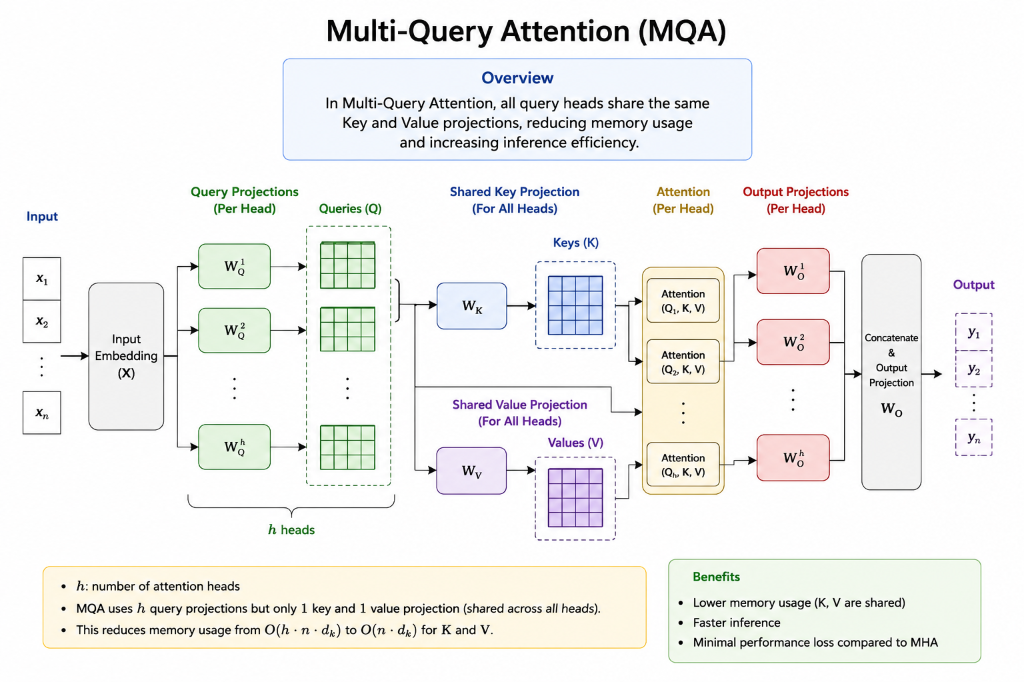
\includegraphics[width=0.95\textwidth]{figures/fig_5_1_gqa.png}
    \caption{Multi-Query Attention (MQA)}
    \label{fig:5_7_mqa}
\end{figure}

\paragraph{Advantages}
\begin{itemize}
    \item Much smaller KV cache
    \item Lower Gpu memory usage
    \item Faster inference
    \item Particularly effective for very LLMs
\end{itemize}

\paragraph{Limitation} Sharing a Single Key and Value across all heads slightly reduces The representational Capacity of The Attention mechanism.

\subsection{II) Grouped-Query Attention (GQA)}

\paragraph{Motivation} MQA greatly reduces memory usage but may sacrifice some modeling capacity because all heads share the same key and value.

GQA provides a compromise between standard multi-head attention and MQA.

\paragraph{Architecture} Instead of one key and value per head or one shared key and value for all heads, attention heads are divided into groups.

Each group shares a key and value projection.

\paragraph{For example} Eight query heads and two KV groups:
\begin{itemize}
    \item Heads 1 to 4: shared $K_1$ and shared $V_1$
    \item Heads 5 to 8: shared $K_2$ and shared $V_2$
\end{itemize}

\begin{figure}[H]
    \centering
    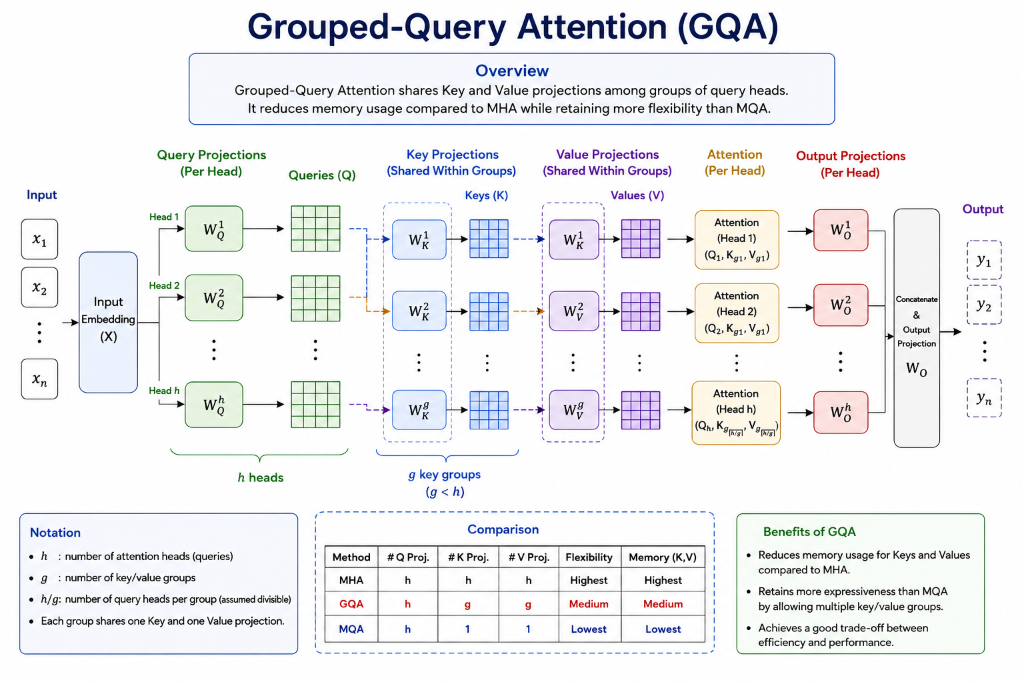
\includegraphics[width=0.95\textwidth]{figures/fig_5_1_mla.png}
    \caption{Grouped-Query Attention (GQA)}
    \label{fig:5_8_gqa}
\end{figure}

\paragraph{Advantages}
\begin{itemize}
    \item Smaller KV cache than Standard Multi-Head Attention
    \item Better modeling capacity than MQA
    \item Excellent balance between memory efficiency and model quality
    \item Widely adopted in modern LLMs
\end{itemize}

\paragraph{Limitation} Although much smaller than standard Multi-Head Attention, The cache remains larger than in MQA.

\subsection{III) Multi-Head Latent Attention (MLA) DeepSeek}

This is currently one of the biggest innovation.

Instead of Storing Keys and Values directly, DeepSeek stores a Compressed latent representation.

\begin{center}
Token $\longrightarrow$ Latent Compression $\longrightarrow$ Small Latent Vector $\longrightarrow$ Cache Latent $\longrightarrow$ when needed Reconstruct $K, V$
\end{center}

So instead of Store $K$ and $V$, DeepSeek stores $z$ (latent vector).

\begin{itemize}
    \item $K$: 512 number, $V$: 512 number, store: 1024 numbers
    \item Latent $\longrightarrow$ 128 numbers
\end{itemize}

Memory is dramatically reduced.

\begin{figure}[H]
    \centering
    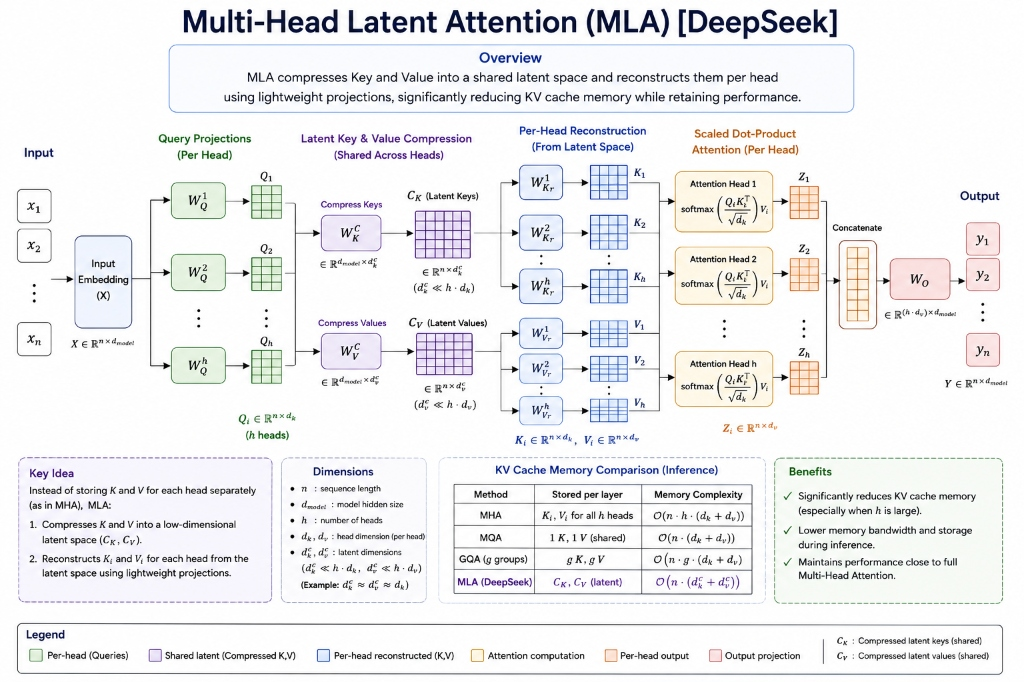
\includegraphics[width=0.98\textwidth]{figures/fig_5_1_comparison.jpg}
    \caption{Multi-Head Latent Attention (MLA) [DeepSeek]}
    \label{fig:5_9_mla}
\end{figure}

\paragraph{Advantages}
\begin{itemize}
    \item Much smaller Kv cache
    \item Longer Context
    \item Better Than GQA for memory
    \item Lower VRAM
    \item Faster inference
\end{itemize}

\begin{figure}[H]
    \centering
    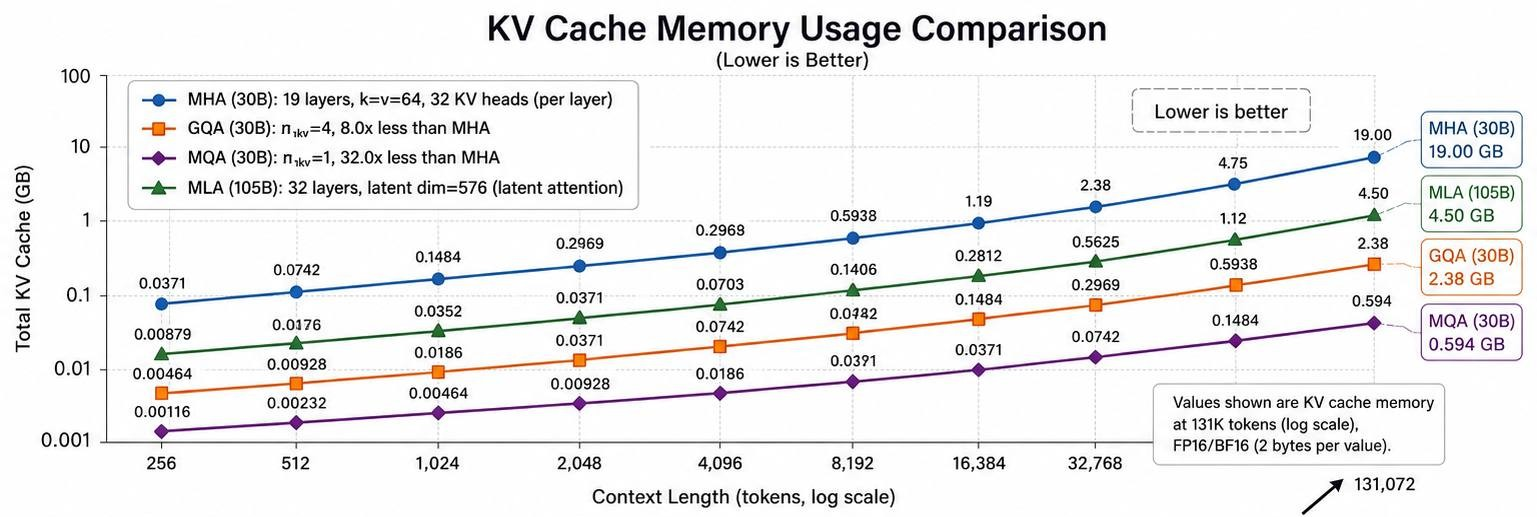
\includegraphics[width=0.95\textwidth]{figures/kv1.jpg}
    \caption{KV Cache Memory Usage Comparison}
    \label{fig:5_6_comparison}
\end{figure}

\begin{figure}[H]
    \centering
    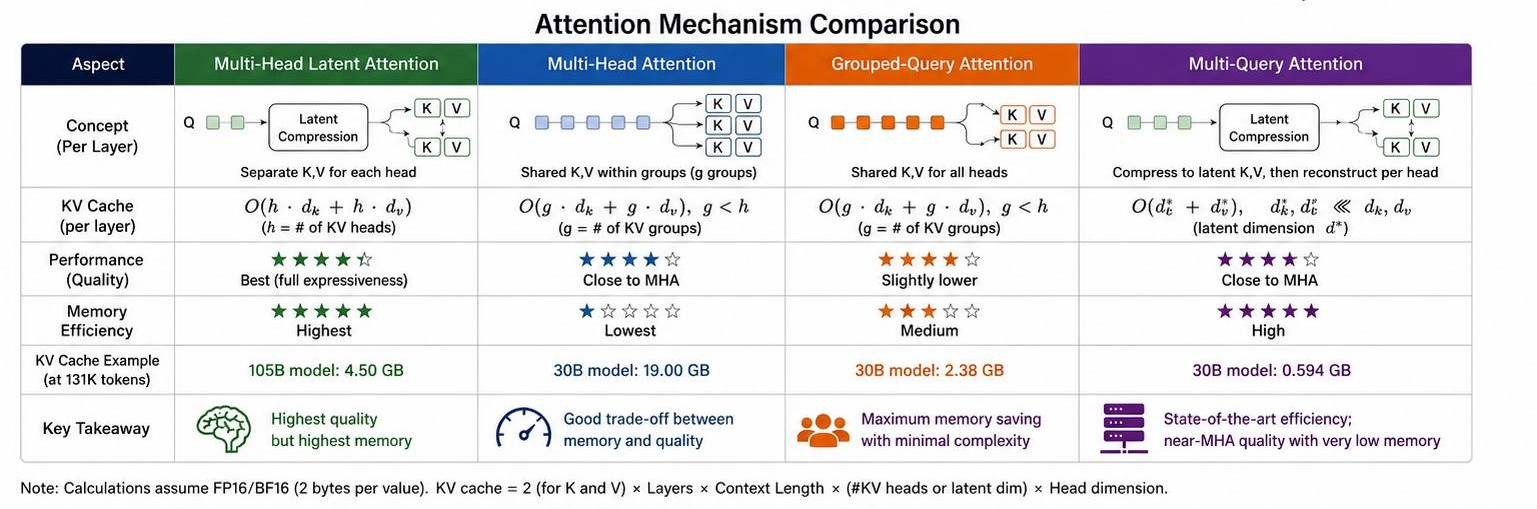
\includegraphics[width=0.95\textwidth]{figures/kv2.jpg}
\end{figure}
\section{Encoder-Only Transformers (BERT Family)}

The Original Transformer was designed for Seq2Seq tasks, where both an encoder and a decoder are required. However, many NLP applications require only language understanding and Never generate new Text as:
\begin{itemize}
    \item Text Classification
    \item Sentiment Analysis
    \item Named Entity Recognition (NER)
    \item Spam detection
    \item Semantic Similarity
    \item Document Classification
\end{itemize}

The Original Transformer (Encoder-Decoder) was Specifically designed for Seq2Seq tasks as machine translation. The researchers recognized That The encoder alone already Produces rich Contextual representations of the input Sequence. Every Encoder layer allows each token to Attend to every other token through bidirectional Self Attention, Producing Contextual embeddings that Capture both local and Global Semantic relationships.

Therefore, if The Goal is to understand text rather Than generate it, The encoder already Provides everything that is needed. This Observation led to a fundamental architecture simplification: Remove the decoder entirely and Retain only the encoder stack.

\subsection{BERT (Bidirectional Encoder Representation from Transformer)}

Based on This idea, Google introduced BERT in 2018 the first Large-scale Pretrained encoder-only Transformer.

BERT consists only of Input $\longrightarrow$ Encoder $\longrightarrow$ Task-specific Output Layer.

The decoder is Completely removed because BERT is designed for understanding rather than generation.

After Several encoder layer, every token contains information from The entire input Sequence. These Contextual embeddings Capture lexical meaning, syntax, semantics and long-range dependencies making them suitable for a wide variety of downstream NLP tasks.

Instead of Generating Text, BERT directly uses these Contextual Representations to make Predictions through a lightweight task-specific output layer.

\paragraph{BERT Architecture}
Unlike the Original Transformer encoder architecture, BERT introduces several modifications to The input representation and training procedure that enable it to learn deep bidirectional contextual representation from Large-scale unlabeled text.

The architecture primarily consists of stacked encoder blocks:
\begin{itemize}
    \item BERT-Base: 12 stacked encoder layers, 12 attention heads and 110 million parameters.
    \item BERT-Large: 24 stacked encoder layers, 16 attention heads and 340 million parameters.
\end{itemize}

BERT introduces a richer input representation by combining token, position, segment embedding:
\begin{equation}
E = E_{\text{token}} + E_{\text{pos}} + E_{\text{segment}}
\end{equation}

BERT Learns Positional Embeddings during Training and produces Contextual representations for every input token which are later used for various downstream NLP tasks.

\subsection{WordPiece Tokenization}

WordPiece Tokenization is a sub-word-based algorithm that enables BERT to efficiently represent text using a fixed-size Vocabulary. By decomposing words into smaller subword units, it Greatly reduces the out-of-vocabulary problem.

Suppose the Vocabulary contains: Play, Playing, Played, Player. Now consider the word playfulness if it not exist in the vocabulary, a word-level Tokenizer cannot represent it and replaces it with \texttt{[unk]}. As a result, all information contained in the word is lost, This Problem is Known as the Out-of-Vocabulary (OOV) problem.

Instead of treating every word as a unique token WordPiece decomposes words into smaller units:
\begin{align*}
\text{Playing} &\longrightarrow \text{Play}, \;\; \text{\#\#ing} \\
\text{Unbelievable} &\longrightarrow \text{un}, \;\; \text{\#\#believ}, \;\; \text{\#\#able}
\end{align*}

The Prefix ""\#\#"" indicates that the Subword Continues the Previous token rather than beginning a new word.

By combining a relatively small set of subwords, WordPiece can represent an enormous number of words, including many that were never seen during training.

Rather than Storing complete words, The Vocabulary contains frequent subwords learned from a large text Corpus. Typical entries include: Play, \texttt{\#\#er}, \texttt{\#\#ing}, \texttt{\#\#ed}, \texttt{\#\#able}, \texttt{\#\#tion}.

For English BERT, the vocabulary contains approximately 30,000 subword tokens. This vocabulary size provides a good balance between representation power and computational efficiency.

\paragraph{Tokenization Process}
The Player is unbelievable. $\longrightarrow$ The, Play, \texttt{\#\#er}, is, un, \texttt{\#\#believ}, \texttt{\#\#able}

Each subword is then mapped to an integer index, which is later converted into a dense embedding vector before entering The Transformer encoder.

If a word cannot be decomposed into Known subwords, it is replaced with The Special token \texttt{[unk]}. However, Because wordPiece can Construct most words from existing subwords, the occurence of \texttt{[unk]} is much lower than in word-level tokenization.

\subsection{Special Tokens and Input Representation}

BERT introduces several Special tokens that Provide structural information and Support different Pretraining and downstream tasks:

\begin{itemize}
    \item \texttt{[cls]}: The beginning of every input sequence, After passing through The encoder, the contextual representation of \texttt{[cls]} is considered a Summary of The entire input Sequence. Instead of Using all token embeddings, many downstream tasks use only The final hidden state of \texttt{[cls]}: $h_{\text{cls}} \in \mathbb{R}^{d_{\text{model}}}$. This vector is passed to a classifier for tasks such as:
    \begin{itemize}
        \item Sentiment Analysis
        \item Spam detection
        \item Topic classification
        \item Next Sentence Prediction
    \end{itemize}
    
    \item \texttt{[SEP]} token (Separator): Marks The end of a sentence or Separate two input sentences: \texttt{[cls]} Question? \texttt{[sep]} Answer \texttt{[sep]}
    
    \item \texttt{[Mask]} token: Is used only during Pretraining. A percentage of input tokens are replaced by \texttt{[mask]}, and The model learns to predict The original words using their surrounding context. \\
    ex: The cat is \texttt{[MASK]} target: Sleeping. \\
    This forms the basis of Masked Language Modeling (MLM) which allows BERT to learn bidirectional Contextual representations. During fine-tuning and inference, The \texttt{[MASK]} token is generally not present, except when performing masked-word prediction tasks.
    
    \item \texttt{[PAD]} token: When Sequences have different lengths, shorter sequences are padded using the \texttt{[PAD]} token.
    \begin{align*}
    \text{Sentence 1}: &\quad \texttt{[cls] I Love AI [SEP]} \\
    \text{Sentence 2}: &\quad \texttt{[cls] Hello . [SEP] [PAD] [PAD]}
    \end{align*}
    Padding ensures that all Sequences in the batch have identical dimension. During Attention computation, Padding tokens are ignored Through an attention mask, Preventing them from influencing the model's Predictions.
\end{itemize}

\subsection{Complete Input Pipeline}

The complete flow of text processing in BERT from raw string to encoder input is presented below:

\begin{figure}[H]
    \centering
    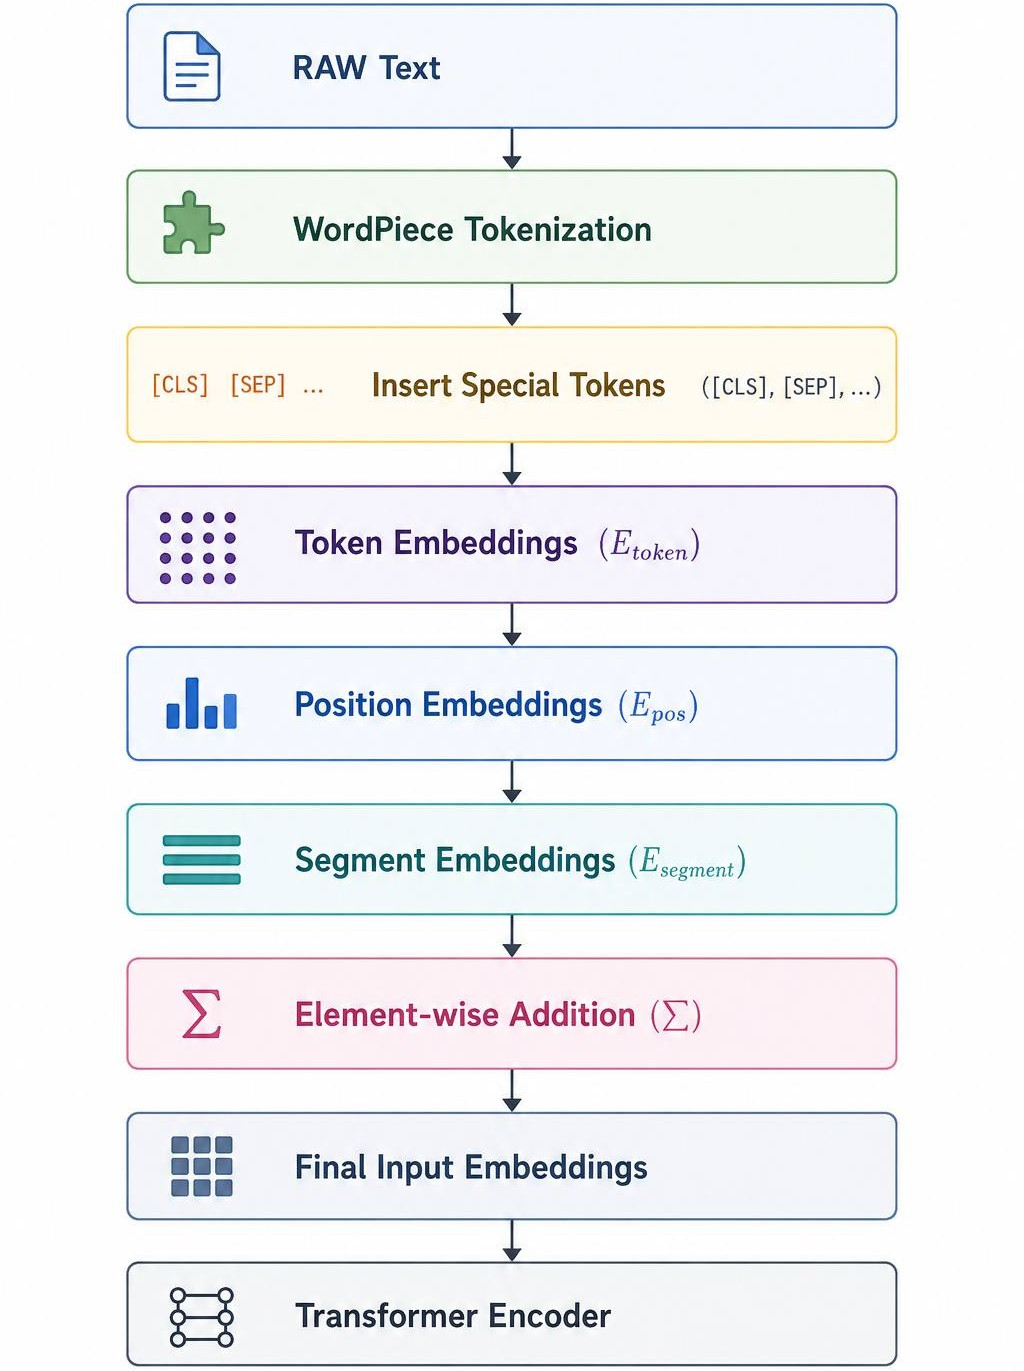
\includegraphics[width=0.95\textwidth]{figures/rnn1.jpg}
\end{figure}

\clearpage
\subsection{Bidirectional Learning}

The defining characteristic of BERT is its ability to learn bidirectional contextual representations. Unlike autoregressive language models, which process text from left to right, BERT simultaneously attends to both the left and right context of every token. This enables the model to construct richer semantic representations and achieve strong performance on language-understanding tasks.

Traditional autoregressive models predict the next token by Considering only the Previous tokens. In Contrast, BERT Processes the entire Sequence simultaneously. Every token can attend to every other token in The Sentence.

\subsection{Next Sentence Prediction (NSP)}

\paragraph{Motivation} Many NLP tasks require understanding the relationship between two sentences rather than a single sentence. Examples include question answering, natural language inference, and semantic similarity.

To Capture These inter-Sentence relationships, BERT introduces Next Sentence Prediction (NSP) as a Second Pretraining Objective.

\paragraph{Training Data Construction}
During Pretraining, The model receives pairs of Sentences.
\begin{itemize}
    \item $50\%$ of The pairs Contain two consecutive sentences from The Original Corpus ($\text{IsNext}$)
    \item $50\%$ Contain two randomly selected, unrelated sentences ($\text{NotNext}$). This creates a balanced binary classification problem.
\end{itemize}

This Creates a balanced binary Classification Problem.

\paragraph{Classification}
After passing through the encoder, the contextual representation of the \texttt{[CLS]} token, $h_{\text{cls}}$, is used as a representation of the entire sentence pair. A linear classifier predicts whether sentence B follows sentence A:
\begin{equation}
P(y) = \text{Softmax}(h_{\text{cls}} W + b)
\end{equation}

\paragraph{Loss function}
NSP is optimized using binary cross-entropy loss:
\begin{equation}
\mathcal{L}_{\text{NSP}} = -y \log(p) - (1-y) \log(1-p)
\end{equation}
\begin{itemize}
    \item $y=1$: for $\text{IsNext}$
    \item $y=0$: for $\text{NotNext}$
\end{itemize}

BERT is trained by optimizing both objectives simultaneously:
\begin{equation}
\mathcal{L} = \mathcal{L}_{\text{MLM}} + \mathcal{L}_{\text{NSP}}
\end{equation}
The encoder parameters are updated jointly using the combined loss.

\subsection{Limitations of NSP}

Subsequent research found that NSP contributed less than initially expected.

The RoBERTa model removed NSP entirely and achieved better performance by training longer on larger datasets.

Although NSP is no longer widely used in modern encoder models, it remains an important component of the original BERT architecture.

Thus, BERT learns both contextual word representations and sentence-level semantics. Although later models demonstrated that NSP is not essential, it played a significant role in the original BERT training procedure.

\subsection{Pretraining Summary}

Before BERT can be applied to downstream tasks such as sentiment analysis and question answering, it undergoes a large-scale pretraining phase. During this stage, the model learns general linguistic knowledge from massive collections of unlabeled text using the self-supervised objectives introduced in MLM (masked language modeling) and NSP (next-sentence prediction).

The result of pretraining is a model that captures grammar, semantics, contextual relationships, and sentence-level information, making it an effective starting point for many NLP applications.

\subsection{Fine-Tuning BERT}

Because BERT has already learned general language representations during pretraining, only a small amount of additional training is needed to specialize these representations for a specific task.

Rather than learning language from scratch, the model learns how to map its existing knowledge to the desired outputs.

Fine-tuning adapts a pretrained BERT model to a specific downstream task using labeled data. During training, both the encoder and the prediction head are optimized jointly, allowing the model to specialize its contextual representations while retaining the linguistic knowledge acquired during pretraining. This transfer-learning approach is one of the main reasons for BERT's effectiveness across a wide range of NLP tasks.

\paragraph{Fine-Tuning Pipeline}
The standard procedure for fine-tuning BERT on downstream tasks is illustrated below:
\begin{figure}[H]
    \centering
    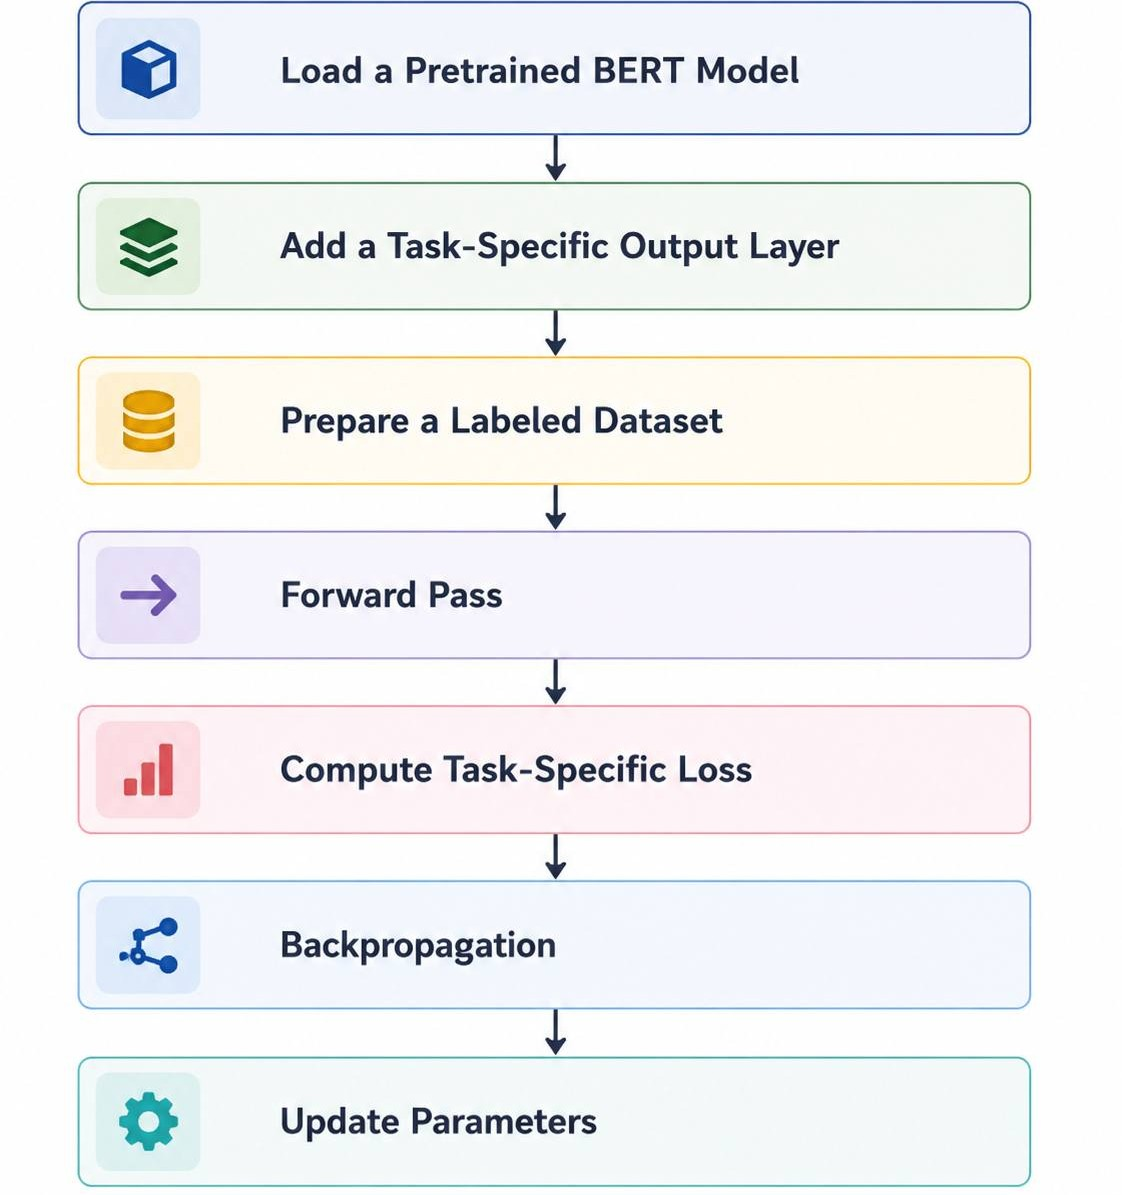
\includegraphics[width=0.95\textwidth]{figures/rnn2.jpg}
\end{figure}
\section{Decoder-Only Transformers (GPT Family)}

The decoder-only architecture emerged from the observation that many applications require only text generation or next-token prediction. The encoder becomes unnecessary, allowing the model to rely solely on the Transformer decoder. This simplification led to the GPT family of models, which has become the dominant architecture for modern large language models because of its scalability, simplicity, and effectiveness in autoregressive text generation.

\subsection{The Limitations of the Original Transformer}

Consider the task of machine Translation:
\begin{equation*}
\text{English} \longrightarrow \text{Encoder} \longrightarrow \text{Context Representation} \longrightarrow \text{Decoder} \longrightarrow \text{French}
\end{equation*}

The decoder requires the encoder because it must generate a sentence based on another input sentence.

Now consider a LLM such as ChatGPT:
\begin{itemize}
    \item Input: Explain what a Transformer is
    \item Desired output: A Transformer is a neural network architecture\dots
\end{itemize}

The model does not transform one sequence into another independent sequence. Instead, it continues the text that already exists: prompt plus generated tokens. No separate encoder source sentence is required.

Because generation depends only on previously generated tokens, the encoder becomes unnecessary.
\begin{itemize}
    \item Since no separate input sequence needs to be encoded, the entire encoder stack can be removed.
    \item The decoder alone is sufficient because it already contains masked self-attention, allowing it to process previously generated tokens while preventing access to future tokens.
\end{itemize}

\subsection{Birth of GPT}

In 2018, OpenAI introduced GPT (Generative Pre-trained Transformer). Unlike BERT, which retained only the encoder, GPT retained only the decoder. Its architecture can be summarized as:
\begin{align*}
\text{Input Token} &\longrightarrow \text{Token Embedding, Positional Embedding} \\
&\longrightarrow \text{Stack of Transformer Decoders} \\
&\longrightarrow \text{Linear Projection} \longrightarrow \text{Softmax} \longrightarrow \text{Next Token Probability}
\end{align*}

The model is trained to repeatedly predict the next token in a sequence using autoregressive language modeling.

The GPT architecture is obtained by simplifying the original Transformer decoder. Since language modeling requires only a single sequence, the encoder is removed, eliminating the need for encoder-decoder (cross-)attention. As a result, queries, keys, and values are all computed from the decoder's hidden representations, leaving masked multi-head self-attention as the only attention mechanism. This simplification reduces computational complexity while preserving the model's ability to generate text autoregressively.

\subsection{Cross Attention Key, Value, Query}

The decoder contains a cross-attention layer that allows it to access the encoder output while generating each token in encoder-decoder Transformers. Queries are computed from the decoder hidden states, whereas keys and values are computed from encoder representations. This enables the decoder to retrieve relevant information from the source sequence throughout generation.

Cross-attention is therefore essential for sequence-to-sequence tasks such as machine translation, where the decoder must continuously reference the encoder input sentence. The main question is: what happens to cross-attention when the encoder is removed in GPT?

GPT is not a sequence-to-sequence model. GPT performs language modeling, where the prompt and generated text belong to the same sequence. Once cross-attention is removed, the only remaining attention mechanism is masked multi-head self-attention. All three matrices are now computed from the decoder hidden states:
\begin{align*}
Q &= X W_Q \\
K &= X W_K \\
V &= X W_V
\end{align*}

Thus, GPT performs self-attention only. Every token attends to previous tokens within the same sequence.

\subsection{The New Decoder Block}

After removing cross-attention, each GPT block contains only two computational sublayers:
\begin{figure}[H]
    \centering
    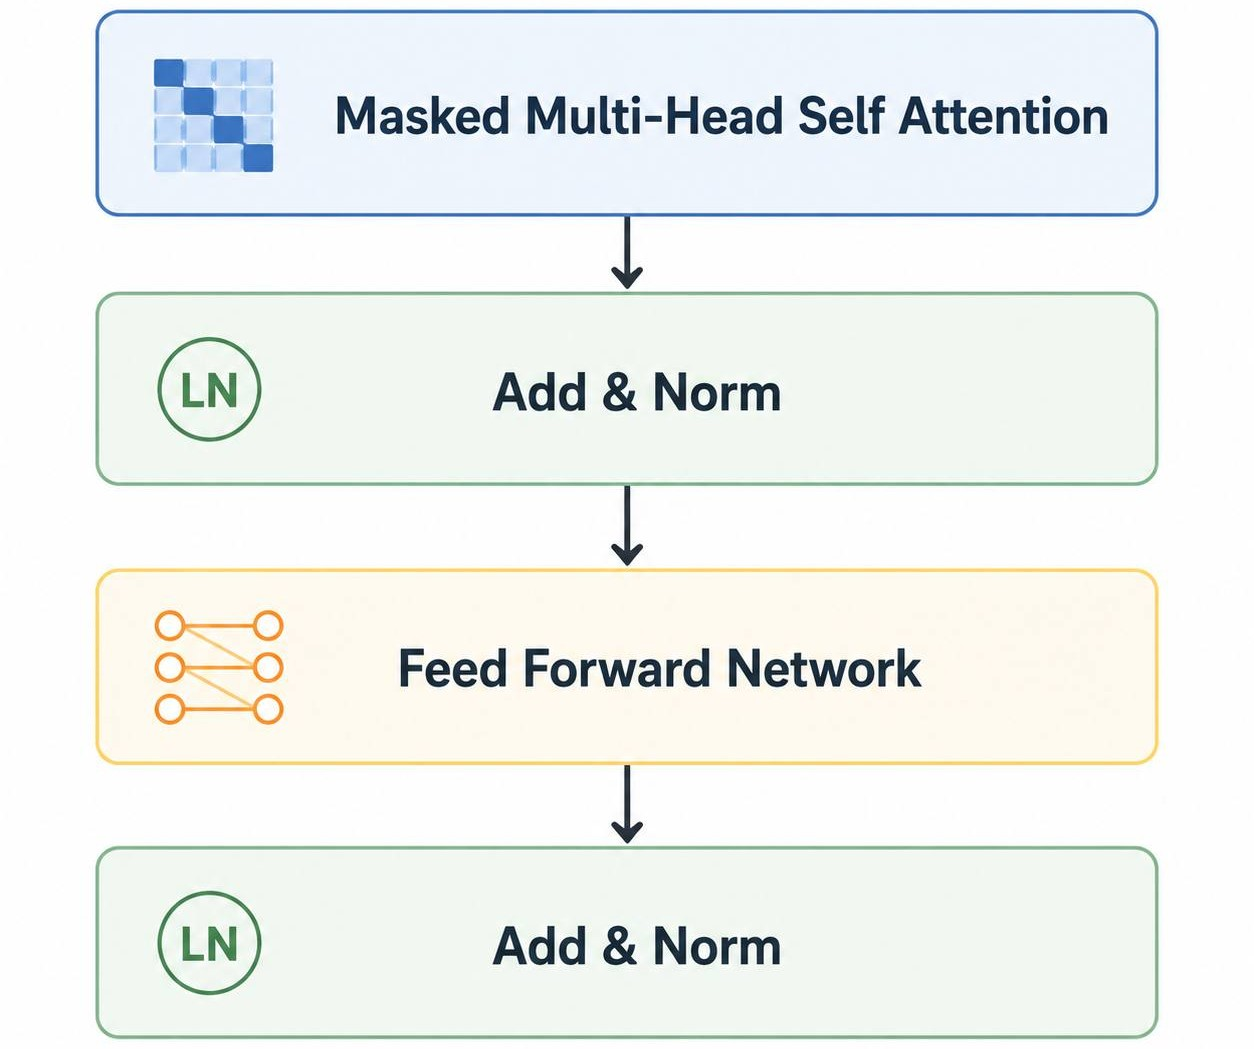
\includegraphics[width=0.95\textwidth]{figures/rnn3.jpg}
\end{figure}


This architecture is considerably simpler than The Original Transformer decoder while Preserving everything required for Autoregressive generation.

At first removing Cross-Attention might Seem like a loss of information. However, GPT does not require information from another Sequence. The Prompt itself becomes part of the decoder input, the Prompt itself provides the Context that would otherwise have been supplied by an encoder.

\subsection{GPT Input Architecture}

GPT converts raw text into numerical representations through tokenization, Vocabulary lookup, token embedding, and positional embedding:
\begin{equation}
E = E_{\text{pos}} + E_{\text{TokenEmb}}
\end{equation}
Unlike BERT, GPT uses only Token and Positional embedding because it Processes a single autoregressive sequence, while early GPT models relied on learnable absolute pos embedding, modern decoder-only models predominantly use Rotary Pos Embedding (RoPE) to Support long-context reasoning and improved positional Generalization.

\subsection{Training GPT}

Unlike traditional supervised learning, GPT does not Require labeled datasets. Instead, the model is trained On large text corpora Collected from sources such as: Books, wikipedia, Scientific Articles, News websites...

Through extensive Optimization over billions to trillions of Tokens, The Model learns General language representations, factual Knowledge, reasoning patterns, and Coding abilities. The resulting foundation model serves as The starting point for subsequent stages such as supervised fine-tuning\dots

\paragraph{Inference}
Autoregressive Generation is The inference Procedure used by GPT and other decoder-only language models. Starting from an input Prompt, The model predicts The one Token at a time, appends it to The Sequence, and repeats The Process until a stopping Condition is reached. Because each prediction depends on all previous tokens, inference is inherently Sequential. Efficient Generation relies on The KV cache.

\subsection{Decoding Algorithms}

After GPT computes The Probability distribution over the Vocabulary, it must choose which token to Generate next. This decision is performed by a decoding algorithm.

\paragraph{Greedy Search}
Always selects The Token with the highest probability. \\
\textit{Limitation:}
\begin{itemize}
    \item Often Produces repetitive Text
    \item Can miss better Overall Sequence
    \item Limited diversity
\end{itemize}

\paragraph{Beam Search}
Maintains the top-$k$ most probable partial Sequences. \\
\textit{Limitation:}
\begin{itemize}
    \item Computationally expensive
    \item Often Generates generic Response
    \item Rarely used in modern LLMs
\end{itemize}

\paragraph{Temperature Sampling}
Control the sharpness of The probability distribution before Softmax:
\begin{itemize}
    \item $0.2 - 0.5$: Factual tasks
    \item $0.7 - 1.0$: Balanced Generation
    \item $+1.2$: Highly Creative generation
\end{itemize}

\paragraph{Top-$K$ Sampling}
Instead of Considering the entire vocabulary, Top-$K$ sampling Keeps only the $K$ most probable tokens. The Remaining tokens receive probability 0, then performed only among these top-$K$ candidates.

\paragraph{Top-$P$ (Nucleus) Sampling}
Instead of Selecting a fixed number of Tokens, Top-$P$ Sampling selects The smallest set of tokens whose cumulative probability exceeds $p$. The candidate set changes dynamically depending On the probability distribution.

\paragraph{Typical Sampling}
Selects tokens whose information content is close to The expected entropy of the Probability distribution, it Prefers tokens that are statistically typical for The Current context.

\paragraph{Repetition Penalty}
During long generation, language models may Repeat words or phrases. A repetition penalty decrease the Probability of tokens that have already appeared in the Generated sequence. This encourages more varied and Coherent Outputs.

\subsection{Combined Decoding Strategies}

Most modern LLMs use a Combination of Decoding techniques rather than a Single algorithm. A Common Combination:
\begin{itemize}
    \item Temperature Sampling
    \item Top-$P$ Sampling
    \item Repetition Penalty
\end{itemize}

This combination provides a good balance between factual accuracy, fluency, and diversity.

\subsection{Best Decoder-Only Models}
\begin{itemize}
    \item ChatGPT
    \item DeepSeek
    \item Claude
    \item LLaMA
    \item Qwen
    \item Grok
\end{itemize}

